\documentclass[noshowpacs,preprintnumbers,amsmath,amssymb, letter]{revtex4}

\usepackage{longtable}%
\usepackage{stmaryrd}%
\usepackage{graphicx}% Include figure files
\usepackage{dcolumn}% Align table columns on decimal point
\usepackage{bm}% bold math
\usepackage{longtable}


\usepackage{float}
\floatstyle{ruled}
\newfloat{codebox}{tb}{los}
\floatname{codebox}{input}
% \renewcommand{\arraystretch}{2}
% \nofiles

\renewcommand{\bfdefault}{b}
\newcommand{\Un}[2]{\mbox{$\mathrm{#1}$ $\mathrm{#2}$}}
\newcommand{\Und}[2]{\mbox{$\mathrm{#1}$-$\mathrm{#2}$}}
\newcommand{\asa}{\textit{ASA}}
\newcommand{\gpIII}{\textit{GENPRO3}}
\newcommand{\ASI}{\lowercase{\emph{a}}-S\lowercase{i}:H}
\newcommand{\CSI}{\emph{c}-Si}
\newcommand{\USI}{$\mu$\lowercase{\emph{c}}-S\lowercase{i}:H}
\newcommand{\Fig}[1]{Fig. \ref{#1}}
\newcommand{\Tab}[1]{Table \ref{#1}}
\newcommand{\Eq}[1]{Eq. (\ref{#1})}
\newcommand{\Sec}[1]{Section \ref{#1}}
\newcommand{\pin}{\emph{pin}}
\newcommand{\ea}{\emph{et al.}}
\newcommand{\vect}[1]{\boldsymbol{#1}}
\newcommand{\version}{0.83}



% correct bad hyphenation here
\hyphenation{op-tical net-works semi-conduc-tor}


\begin{document}
\title{PVMOS manual - Version \version}

\author{B.E. Pieters}%
\email{b.pieters@fz-juelich.de}
\affiliation{Institut f\"ur Energie und Klimaforschung - IEK5 Photovoltaik, Forschungszentrum J\"ulich, 52425 J\"ulich, Germany}
\date{\today}
\maketitle

\section{Introduction}
This is the manual for the Photo-Voltaic MOdule Simulator (PVMOS). PVMOS is an ordinary differential equation solver using finite-differences specifically designed to electrically model solar modules. For more information on how that works I refer the reader to \cite{pvmos:2014}. The purpose of this document is to document how PVMOS is operated and installed. In the following sections I discuss in order, the installation, basic usage and operating principles and finally a detailed discussion of all available functions.

\section{Disclaimer}
If this software ever does anything you think I claim it does or should do, consider yourself lucky.\\ \\
\texttt{
PVMOS  Copyright (C) 2014  B. E. Pieters\\
This program comes with ABSOLUTELY NO WARRANTY. This is free software, and you are welcome to\\
redistribute under certain conditions. You should have received a copy of the GNU General \\
Public License along with this program. If not, see <http://www.gnu.org/licenses/>.\\
}\\

\section{What is PVMOS}
In its essence PVMOS is a Poisson solver. The Poisson equation is solved for several stacked, 2D ``electrodes'', where each electrode is coupled to the electrodes above and below (note that a stack of 2D electrodes makes a 3D structure). The electrodes itself are simply conductors and behave linearly (Ohmic). However, the connection between the electrodes can be non-linear (e.g. a diode). Now, there are several limitations of the structures that PVMOS handles. The main limitation is that the meshes are 2D as in PVMOS all electrodes share the same 2D mesh. This means that PVMOS is specifically designed for flat layered structures. PVMOS uses straight forward finite-differences to solve the coupled Poisson equations. As such the 2D meshes in PVMOS divide the 2D surface in rectangular elements. Now every element in the mesh must be associated with certain properties. Storing properties on a per element basis would put a heavy burden on the memory resources. For that reason elements are grouped into ``areas'' where each area constitutes a certain combination of properties. A mesh therefore also contains a list of all areas and every element is a member of one of the areas in the mesh (note that an element is always assigned to one area, i.e. you need at least one area for every unique combination of local properties). Also note that as all electrodes share the same 2D mesh, one area contains the properties for all electrodes and connections between them.

PVMOS is a commandline program which must be given an file. The PVMOS input file is processed sequentially and contains commands that create or modify meshes, perform a simulation, or export data to a file. A complete list of commands is presented in Section \ref{commref}. In PVMOS we can define more than one mesh at the same time. This is useful as it allows you to create new meshes by joining two meshes, e.g., to create several series connected cells in a thin-film module. In order to reference one particular mesh, each mesh has a name. This name must thus be provided to any command that operates on a mesh. Likewise, some commands operate on an area within a mesh and thus areas also have a name. To reference an area within a mesh we use the following syntax \texttt{<mesh-name>.<area-name>}, i.e. the name of the mesh followed by a dot and the name of the area within that particular mesh. Sometimes we need to select elements in a mesh (for example when we want to assign a set of elements to a certain area). To this end each mesh has a list of selected elements. If you select elements in a mesh the list is occupied by the element ID's, after which you can do operations on the selected elements. Note that elements are selected on a per mesh basis.

It may be useful to store intermediate results, especially as sometimes creating the mesh may take some time and you want to do many different calculations based on the same mesh. For such cases PVMOS has a binary file format to store complete meshes with all elements, areas, properties and simulation results. This mesh may be loaded later to continue where you left of. The primary focus is to store intermediate results and as such not much value is put on compatibility between different PVMOS versions, i.e. compatibility between the file format of different PVMOS versions is not guaranteed (in general compatibility will break if a new version makes any change in the mesh data structures). The binary format is also used for a dynamic library for GNU Octave (an open source tool largely compatible with Matlab), which allows you to generate a mesh for PVMOS within octave and store it in binary form for use in PVMOS. 

\section{Basic Usage}
The input for PVMOS is a plain text file with commands. To solve a problem PVMOS is typically called from the command line with as an argument the file name describing the problem. With these input files you can specify the geometry of your solar cell/module including the local properties such as electrode sheet resistances and solar cell properties. You can also specify which calculations you want PVMOS should perform and what data to save. A call to PVMOS from the command line looks like this
\begin{verbatim}
pvmos [options/variables] <input-file>
\end{verbatim}
where the optional argument \texttt{[options/variables]} is used to set options and define variables. Valid options and variable definitions are:
\begin{itemize}
\item{``-q''} Set verbosity level to quiet (i.e. supress all non essential output)
\item{``-n''} Set verbosity level to normal 
\item{``-v''} Set verbosity level to verbose
\item{``-db''} Set verbosity level to debug
\item{``-vf''} Indicates next argument is a variable file
\item{``\textless name\textgreater=\textless value\textgreater''} Define variable \textless name\textgreater. Note there should be no white spaces within the definition
\end{itemize}
A variable file is a file with one variable per line of the form ``\textless name\textgreater=\textless value\textgreater''. In variable files all spaces are ignored. Lines that do not follow this format are ignored. Note that not all variable names are allowed, see Section \ref{expressions}. The last option must be the PVMOS input file, a plain text input file with commands for PVMOS.

\section{Installation Instructions}	
PVMOS is a command-line application written entirely in C. For the operation PVMOS depends on several libraries, most notably \texttt{cholmod}, for the solving of sparse linear systems. PVMOS has been tested on Linux and Windows systems. To install PVMOS you need to either compile the source, for which a Makefile is provided, or you need to download pre-compiled binaries for your system (if available). 

\subsection{Compiling from source}
Here are the instructions to compile the PVMOS executable:
\begin{enumerate}
\item{} Install PVMOS's dependencies (\texttt{BLAS} and \texttt{CHOLMOD}). These libraries should be readily available in most linux distributions. Take care to install the development files (i.e. headers) for these libraries too 
\item{} Edit the Makefile, in particular you may have to change the BLAS library to link to (the used BLAS library has a relatively large impact on performance, see below) or change the install directory
\item{} type ``make'', and ``make install''
\end{enumerate}

The performance of PVMOS is typically strongly dependent on the performance of the sparse linear solver (i.e. \texttt{cholmod}). For an optimal performance an optimized \texttt{BLAS} library must be used (the reference \texttt{BLAS} is comparatively slow). For an optimized \texttt{BLAS} there are several options. One option is to use ATLAS which is available for all common CPU architectures and gives a decent performance. On some architectures you can use \texttt{OpenBLAS} (\texttt{OpenBLAS} is an actively developed fork of the now unmaintained \texttt{GoTo BLAS}), which generally performs better than ATLAS. Some CPU manufacturers also publish their own optimized \texttt{BLAS} libraries for their CPU's (e.g. Intel and AMD). Per default the make-files are set up to use \texttt{OpenBLAS} as it provides a good performance on the most common desktop CPU architectures and is freely available.

\subsection{Pre-compiled binaries (Windows)}
There are two pre-compiled versions for windows, 32 and 64 bit. If your system supports it I suggest to use 64 bit as 32 bit applications are rather limited in the maximum allocatable memory space (< 2Gb), you may run into this limit for larger problems. The binary distribution consists of an executable with several dll's. The installation procedure for PVMOS manual as no installer is provided (you can help PVMOS by making one). So here is the procedure for a binary install:
\begin{enumerate}
\item{} Download the binary 
\item{} Unpack the files in a directory of your choise
\item{} Optional: Add the path to your PVMOS executable to the PATH variable
\end{enumerate}

\subsubsection{Setting the ``PATH'' variable}
A properly set PATH variable will allow you to execute PVMOS from the command line without typing the full path to the PVMOS executable. Here I describe how to edit your path variable in Windows 7. First another word of warning. Adding things to the path variable is mostly harmless, however, if you break your path string (e.g. delete a part) you may seriously impair the functioning of programs that need the path variable. Follow these instructions on your own risk!
\begin{enumerate}
\item{} Click on the start menu 
\item{} type ``PATH'' in the ``search programs and files'' field, you should now find options to edit the path variable for the system of for the current user, select to edit it for the current user
\item{} Select the path variable
\item{} Click on Edit
\item{} Scroll to the end of the string and add \texttt{;<installation directory>}, where \texttt{<installation directory>} points to the location of your PVMOS executable
\item{} Click on OK
\item{} Click on OK
\end{enumerate}

\subsection{Installing the GNU-Octave PVMOS-mesh package}
The PVMOS package for GNU Octave is a set of tools to create and save binary PVMOS meshes from within GNU Octave. A more detailed description of the package can be found in Section \ref{mkpvmosmesh}. Installing the PVMOS package in Octave is through the ``pkg'' command, i.e. the usual procedure to install packages in GNU Octave. Prepared packages are available for download and are named PVMOS-mesh-<version>.tar.gz. The package can also be created from source using ``make PVMOS-mesh.pkg''. After installing the package you can use ``pkg load PVMOS-mesh'' to load the functions for use.

\section{Recommended software}
Obviously you are free to use whatever software you want. However, to process data from PVMOS or to get data into PVMOS I often use file formats which will not be supported by all software packages. I thus here detail my software setup in the hope it helps you. All software here is free and open source software.

\subsection{Get data into PVMOS: GNU Octave \& Inkscape}
These programs are useful when defining complex geometries. If you want to define complex geometries in PVMOS there are basically three ways:
\begin{enumerate}
\item{} Use the PVMOS scripting language. The advantages of this method is that it can be very accurate and fast and is independent of any other software, the downside is that it quickly becomes tedious
\item{} mkpvmosmesh with GNU Octave. This allows you to use all the data and image processing power of Octave to generate meshes. However, this library only allows you to create mesh topologies consisting of rows and columns (i.e. meshes easily defined with a matrix
\item{} Define geometries using polygons. PVMOS has good support for polygons to select and specify various areas in your device. Complicated shapes may be created in a graphics program such as inkscape and exported to PVMOS. For this I have an extension to export data from inkscape for use in PVMOS. In combination with the trace bitmap feature of inkscape you can quickly define appropriate polygons for complicated geometries if you provide a bitmap image, e.g. you can create a polygon for the metalization pattern of a device by tracing a picture. This method potentially has a lower memory footprint compared to the GNU Octave option. 
\end{enumerate}   

Inkscape is a powerful vector graphics tool. One of the graphics objects Inkscape supports are ``paths''. In its simplest form a path is simply a polygon. As PVMOS can use polygons when defining a mesh it makes sense to use a tool such as Inkscape to create the polygons as Inkscape provides a powerful, graphical, means to do so. In order to get the polygon data out of inkscape I created a simple extension which extracts the data out of a polygon. To use this extension select a path with polygon data and select the ExportXY extension, a popup window will come up with coordinates you can select and paste in a polygon data file. Note however that Inkscape paths may also be bezier curves, which PVMOS does not support. To use the extension is is thus required that the path data is forced to be a polygon. For this you can use the flatten Bezier extension in Inkscape. I have not fully dug into Inkscape's internal units. This can be tricky as Inkscape may use all sorts of transforms on objects. This means that the polygon data may need to be scaled, rotated, mirrored and shifted to get the data in the correct unit. For this I provide a small CLI program ``transformpolygon''. 


\subsection{Analyse simulated data: Gnuplot}
The data-format that PVMOS uses for element-wise data export is laid out such that Gnuplot can make sense out of the data. Other plotting tools may not support this format. The element-wise data export allows you to export data from the mesh on a per-element basis and is particularly useful for inspecting meshes to ensure a correct mesh definition. For this reason I recommend the use of Gnuplot. Other data formats that PVMOS should not be a problem for other plotting tools.

\section{\label{syntax}PVMOS input file format}
\subsection{\label{commref}Command Reference}
\begin{longtable}{p{0.2\textwidth}p{0.8\textwidth}}
\multicolumn{2}{l}{\textsc{Creating Meshes}} \\*
\hline
Keyword & Description \\
\hline\\
\texttt{newmesh} 	& Create a new, rectangular mesh. The command takes seven arguments:
\begin{enumerate}
\item \texttt{x1}, x-coordinate of the lower left corner
\item \texttt{y1}, y-coordinate of the lower left corner
\item \texttt{x2}, x-coordinate of the upper right corner
\item \texttt{y2}, y-coordinate of the upper right corner
\item \texttt{Nx}, Number of elements in x direction
\item \texttt{Ny}, Number of elements in y direction
\item \texttt{mesh-name}, Name of the new mesh
\end{enumerate}\\
%%%%%%%%%%%%%%%%%%%%%%%%%%%%%%%%%%%%%%%%%%%%%%%%%%%%%%%%%%%%%%%%%%%%%%%%%
\texttt{addcol\_left} 	& Add a column of elements to the left side of a mesh. This command requires the mesh has no holes and the left side of the mesh is flat, i.e. the left edge is vertical. This command will add one element to the left of each element at the left edge of the mesh. The newly added elements inherit all properties from the element on their right. The command takes two arguments:
\begin{enumerate}
\item \texttt{mesh-name}, Name of the new mesh
\item \texttt{dx}, width of the column to be added. 
\end{enumerate}\\
%%%%%%%%%%%%%%%%%%%%%%%%%%%%%%%%%%%%%%%%%%%%%%%%%%%%%%%%%%%%%%%%%%%%%%%%%
\texttt{addcol\_right} 	& Add a column of elements to the right side of a mesh. This command requires the mesh has no holes and the right side of the mesh is flat, i.e. the right edge is vertical. This command will add one element to the right of each element at the right edge of the mesh. The newly added elements inherit all properties from the element on their left. The command takes two arguments:
\begin{enumerate}
\item \texttt{mesh-name}, Name of the new mesh
\item \texttt{dx}, width of the column to be added. 
\end{enumerate}\\
%%%%%%%%%%%%%%%%%%%%%%%%%%%%%%%%%%%%%%%%%%%%%%%%%%%%%%%%%%%%%%%%%%%%%%%%%
\texttt{addrow\_top} 	& Add a row of elements to the top side of a mesh. This command requires the mesh has no holes and the top side of the mesh is flat, i.e. the top edge is horizontal. This command will add one element on top of each element at the top edge of the mesh. The newly added elements inherit all properties from the element below. The command takes two arguments:
\begin{enumerate}
\item \texttt{mesh-name}, Name of the new mesh
\item \texttt{dy}, width of the row to be added. 
\end{enumerate}\\
%%%%%%%%%%%%%%%%%%%%%%%%%%%%%%%%%%%%%%%%%%%%%%%%%%%%%%%%%%%%%%%%%%%%%%%%%
\texttt{addrow\_bottom} 	& Add a row of elements below a mesh. This command requires the mesh has no holes and the bottom side of the mesh is flat, i.e. the bottom edge is horizontal. This command will add one element below each element at the bottom edge of the mesh. The newly added elements inherit all properties from the element above it. The command takes two arguments:
\begin{enumerate}
\item \texttt{mesh-name}, Name of the new mesh
\item \texttt{dy}, width of the row to be added. 
\end{enumerate}\\
%%%%%%%%%%%%%%%%%%%%%%%%%%%%%%%%%%%%%%%%%%%%%%%%%%%%%%%%%%%%%%%%%%%%%%%%%
\texttt{joinmesh}	& Create new mesh by joining two meshes. Make sure the meshes touch but do not overlap. The function takes offset values as input which allow you to "shift" the second mesh to align it to the first. The command takes 5 arguments:
\begin{enumerate}
\item \texttt{x\_off}, x-offset in coordinate system of the second mesh
\item \texttt{y\_off}, y-offset in coordinate system of the second mesh 
\item \texttt{mesh1-name}, Name of the first mesh
\item \texttt{mesh2-name}, Name of the second mesh
\item \texttt{mesh3-name}, Name of the resulting mesh
\end{enumerate}\\
%%%%%%%%%%%%%%%%%%%%%%%%%%%%%%%%%%%%%%%%%%%%%%%%%%%%%%%%%%%%%%%%%%%%%%%%%
\texttt{joinmesh\_h}	& Create new mesh by joining two meshes. Make sure the meshes touch but do not overlap. The function takes a y-offset value as input which allow you to "shift" the second mesh in the y-direction to align it to the first. The x-offset value is the maximal x-value found in the first mesh. The command takes 4 arguments:
\begin{enumerate}
\item \texttt{y\_off}, y-offset in coordinate system of the second mesh 
\item \texttt{mesh1-name}, Name of the first mesh
\item \texttt{mesh2-name}, Name of the second mesh
\item \texttt{mesh3-name}, Name of the resulting mesh
\end{enumerate}\\
%%%%%%%%%%%%%%%%%%%%%%%%%%%%%%%%%%%%%%%%%%%%%%%%%%%%%%%%%%%%%%%%%%%%%%%%%
\texttt{joinmesh\_v}	& Create new mesh by joining two meshes. Make sure the meshes touch but do not overlap. The function takes an x-offset value as input which allow you to "shift" the second mesh in the x-direction to align it to the first. The y-offset value is the maximal y-value found in the first mesh. The command takes 4 arguments:
\begin{enumerate}
\item \texttt{x\_off}, x-offset in coordinate system of the second mesh 
\item \texttt{mesh1-name}, Name of the first mesh
\item \texttt{mesh2-name}, Name of the second mesh
\item \texttt{mesh3-name}, Name of the resulting mesh
\end{enumerate}\\
\texttt{dupmesh}	& Duplicate a mesh. The command takes 2 arguments:
\begin{enumerate}
\item \texttt{mesh1-name}, Name of the mesh to be duplicated
\item \texttt{mesh2-name}, Name of the resulting copy
\end{enumerate}\\
\texttt{add\_electrode}	& Adds an electrode to a certain mesh. The command takes one argument:
\begin{enumerate}
\item \texttt{mesh-name}, Name of the mesh
\end{enumerate}\\
%%%%%%%%%%%%%%%%%%%%%%%%%%%%%%%%%%%%%%%%%%%%%%%%%%%%%%%%%%%%%%%%%%%%%%%%%
\multicolumn{2}{l}{\textsc{Transforming Meshes}} \\*
\hline
Keyword & Description \\
\hline\\
%%%%%%%%%%%%%%%%%%%%%%%%%%%%%%%%%%%%%%%%%%%%%%%%%%%%%%%%%%%%%%%%%%%%%%%%%
\texttt{move} 	& Move a mesh in x- and y-directions. The command takes three arguments:
\begin{enumerate}
\item \texttt{mesh-name}, Name of the mesh
\item \texttt{delta x}, move distance in x-direction
\item \texttt{delta y}, move distance in y-direction
\end{enumerate}\\
%%%%%%%%%%%%%%%%%%%%%%%%%%%%%%%%%%%%%%%%%%%%%%%%%%%%%%%%%%%%%%%%%%%%%%%%%
\texttt{rotate} 	& Rotate mesh around a center coordinate. Rotation can only be performed over multiples of 90 degrees. The command takes four arguments:
\begin{enumerate}
\item \texttt{mesh-name}, Name of the mesh
\item \texttt{x}, x-coordinate of rotation center
\item \texttt{y},y-coordinate of rotation center
\item \texttt{d}, degrees to rotate over (must be a multiple of 90)
\end{enumerate}\\
%%%%%%%%%%%%%%%%%%%%%%%%%%%%%%%%%%%%%%%%%%%%%%%%%%%%%%%%%%%%%%%%%%%%%%%%%
\texttt{flipx} 	& Mirror a mesh in the y-axis. The command takes one argument:
\begin{enumerate}
\item \texttt{mesh-name}, Name of the mesh
\end{enumerate}\\
%%%%%%%%%%%%%%%%%%%%%%%%%%%%%%%%%%%%%%%%%%%%%%%%%%%%%%%%%%%%%%%%%%%%%%%%%
\texttt{flipy} & Mirror a mesh in the x-axis. The command takes one argument:
\begin{enumerate}
\item \texttt{mesh-name}, Name of the mesh
\end{enumerate}\\
%%%%%%%%%%%%%%%%%%%%%%%%%%%%%%%%%%%%%%%%%%%%%%%%%%%%%%%%%%%%%%%%%%%%%%%%%
\texttt{scale} 	& Scale all coordinates in a mesh. The command takes two arguments:
\begin{enumerate}
\item \texttt{mesh-name}, Name of the mesh
\item \texttt{f}, scaling factor
\end{enumerate}\\
%%%%%%%%%%%%%%%%%%%%%%%%%%%%%%%%%%%%%%%%%%%%%%%%%%%%%%%%%%%%%%%%%%%%%%%%%
\texttt{scalex} 	& Scale all x-coordinates in a mesh. The command takes two arguments:
\begin{enumerate}
\item \texttt{mesh-name}, Name of the mesh
\item \texttt{f}, scaling factor
\end{enumerate}\\
%%%%%%%%%%%%%%%%%%%%%%%%%%%%%%%%%%%%%%%%%%%%%%%%%%%%%%%%%%%%%%%%%%%%%%%%%
\texttt{scaley} 	& Scale all y-coordinates in a mesh. The command takes two arguments:
\begin{enumerate}
\item \texttt{mesh-name}, Name of the mesh
\item \texttt{f}, scaling factor
\end{enumerate}\\
%%%%%%%%%%%%%%%%%%%%%%%%%%%%%%%%%%%%%%%%%%%%%%%%%%%%%%%%%%%%%%%%%%%%%%%%%
\texttt{boundingbox} 	& Change the mesh bounding box. This argument scales and moves a mesh such that it fits in a specified rectangle (the bounding box). The mesh is either scaled preserving the aspect ratio or without preserving it. The command takes six arguments:
\begin{enumerate}
\item \texttt{mesh-name}, Name of the mesh
\item \texttt{x1}, x-coordinate of the lower left corner of the bounding box
\item \texttt{y1}, y-coordinate of the lower left corner of the bounding box
\item \texttt{x2}, x-coordinate of the upper right corner of the bounding box
\item \texttt{y2}, y-coordinate of the upper right corner of the bounding box
\item \texttt{R}, Argument can be either 0, do not preserve mesh aspect ratio, or 1, preserve mesh aspect ratio. 
\end{enumerate}\\
%%%%%%%%%%%%%%%%%%%%%%%%%%%%%%%%%%%%%%%%%%%%%%%%%%%%%%%%%%%%%%%%%%%%%%%%%
\multicolumn{2}{l}{\textsc{Selecting Elements}} \\*
\hline
Keyword & Description \\
\texttt{select\_rect}	& Select a rectangular area in a mesh. If currently nodes are already selected in the mesh, the command selects the subset of selected nodes within the rectangle. If the latter is not desired use deselect first. The command takes five arguments:
\begin{enumerate}
\item \texttt{x1}, x-coordinate of the lower left corner of the selected rectangle
\item \texttt{y1}, y-coordinate of the lower left corner of the selected rectangle
\item \texttt{x2}, x-coordinate of the upper right corner of the selected rectangle
\item \texttt{y2}, y-coordinate of the upper right corner of the selected rectangle
\item \texttt{mesh-name}, Name of the mesh
\end{enumerate}\\
%%%%%%%%%%%%%%%%%%%%%%%%%%%%%%%%%%%%%%%%%%%%%%%%%%%%%%%%%%%%%%%%%%%%%%%%%
\texttt{select\_rect\_contour}	& Select the contour of a rectangle in a mesh. If currently nodes are already selected in the mesh, the command selects the subset of selected nodes within the rectangle. If the latter is not desired use deselect first. The command takes six arguments:
\begin{enumerate}
\item \texttt{x1}, x-coordinate of the lower left corner of the selected rectangle
\item \texttt{y1}, y-coordinate of the lower left corner of the selected rectangle
\item \texttt{x2}, x-coordinate of the upper right corner of the selected rectangle
\item \texttt{y2}, y-coordinate of the upper right corner of the selected rectangle
\item \texttt{d}, distance from the contour within which elements are selected
\item \texttt{mesh-name}, Name of the mesh
\end{enumerate}\\
%%%%%%%%%%%%%%%%%%%%%%%%%%%%%%%%%%%%%%%%%%%%%%%%%%%%%%%%%%%%%%%%%%%%%%%%%
\texttt{select\_circ}	& Select a circular area in a mesh. If currently nodes are already selected in the mesh, the command selects the subset of selected nodes within the circle. If the latter is not desired use deselect first. The command takes four arguments:
\begin{enumerate}
\item \texttt{x\_c}, center x-coordinate of the selected circle
\item \texttt{y\_c}, center y-coordinate of the selected circle
\item \texttt{r}, radius of the selected circle
\item \texttt{mesh-name}, Name of the mesh
\end{enumerate}\\
%%%%%%%%%%%%%%%%%%%%%%%%%%%%%%%%%%%%%%%%%%%%%%%%%%%%%%%%%%%%%%%%%%%%%%%%%
\texttt{select\_circ\_contour}	& Select the contour of a circle in a mesh. If currently nodes are already selected in the mesh, the command selects the subset of selected nodes within the circle. If the latter is not desired use deselect first. The command takes five arguments:
\begin{enumerate}
\item \texttt{x\_c}, center x-coordinate of the selected circle
\item \texttt{y\_c}, center y-coordinate of the selected circle
\item \texttt{r}, radius of the selected circle
\item \texttt{d}, distance from the contour within which elements are selected
\item \texttt{mesh-name}, Name of the mesh
\end{enumerate}\\
%%%%%%%%%%%%%%%%%%%%%%%%%%%%%%%%%%%%%%%%%%%%%%%%%%%%%%%%%%%%%%%%%%%%%%%%%
\texttt{select\_poly}	& Select an area within a polygon-contour. In order to use this command you must first load or define a polygon from file with the \texttt{load\_poly} or \texttt{define\_poly} commands. If currently elements are already selected in the mesh, the command selects the subset of selected elements within the polygon. If the latter is not desired use deselect first. If a polygon circles an element more than once the node is selected if the node is circled an uneven number of times. This allows one to define polygon areas with holes. To make a hole, define one outer part of the polygon and one inner part and have a break between these tho parts, i.e. the two parts should not be connected by a line segment, (see \texttt{load\_poly} and \texttt{loaddefine\_poly}). The command takes one argument.
\begin{enumerate}
\item \texttt{mesh-name}, Name of the mesh
\end{enumerate}\\
%%%%%%%%%%%%%%%%%%%%%%%%%%%%%%%%%%%%%%%%%%%%%%%%%%%%%%%%%%%%%%%%%%%%%%%%%
\texttt{select\_poly\_contour}	& Select an area around a polygon-contour. In order to use this command you must first load or define a polygon from file with the \texttt{load\_poly} or \texttt{define\_poly} commands. If currently elements are already selected in the mesh, the command selects the subset of selected elements near to the polygon. If the latter is not desired use deselect first. This command is often useful to refine the mesh along the polygon before using \texttt{select\_poly} to assign elements to a new area. It may also be useful to define things such as cracks. If no line segment is present between two seubsequent coordinates in the polygon (i.e. a break in the polygon), no nodes are selected between these coordinates. The command takes three arguments.
\begin{enumerate}
\item \texttt{distance}, Distance from the polygon
\item \texttt{loop}, Argument takes either 0 (not looped) or 1 (looped). In looped modus the last point in the polygon is connected to the first point.
\item \texttt{mesh-name}, Name of the mesh
\end{enumerate}\\
%%%%%%%%%%%%%%%%%%%%%%%%%%%%%%%%%%%%%%%%%%%%%%%%%%%%%%%%%%%%%%%%%%%%%%%%%
\texttt{load\_poly}	& Load a polygon from file. This command is used in conjunction with the \texttt{select\_poly} and the \texttt{select\_poly\_contour} commands. Once a polygon is loaded you can use it to select until a new \texttt{load\_poly} command is given. Polygons may contain breaks (i.e. absence of a line segment between two coordinates). The command takes one argument.
\begin{enumerate}
\item \texttt{file-name}, Name of the file describing the polygon (one 2D coordinate per line, i.e., two columns, 1: x-coordinate, 2: y-coordinate, empty lines indicate a break)
\end{enumerate}\\
%%%%%%%%%%%%%%%%%%%%%%%%%%%%%%%%%%%%%%%%%%%%%%%%%%%%%%%%%%%%%%%%%%%%%%%%%
\texttt{define\_poly}	& Define polygon within the input file. See also the \texttt{load\_poly} command for an alternative method. The difference between this command and the \texttt{load\_poly} command is that with this command you can define the polygon within the PVMOS input file. As such it is best suited for simple polygons. The \texttt{define\_poly} command marks the start and the end of a table defining the polygon. Between the two \texttt{define\_poly} commands, one coordinate (x- and y-value) per line is expected and an empty line indicates a break, i.e.,\\
&
\begin{tabular}{ll}
	\texttt{define\_poly} \\
	$x_1$ & $y_1$ \\
	$x_2$ & $y_2$ \\
	$x_3$ & $y_3$ \\
	... & ... \\
	$x_N$ & $y_N$ \\
	\\
	$x_{N+1}$ & $y_{N+1}$ \\
	... & ... \\
	$x_M$ & $y_M$ \\
	\texttt{define\_poly} \\
\end{tabular}\\
&where $(x_i,y_i)$ is the $i$-th coordinate of the polygon and between coordinates $N$ and $N+1$ there is a break.\\
%%%%%%%%%%%%%%%%%%%%%%%%%%%%%%%%%%%%%%%%%%%%%%%%%%%%%%%%%%%%%%%%%%%%%%%%%
\texttt{select\_area}	& Select all nodes assigned to a given area. If currently nodes are already selected in the mesh, the command selects the subset of selected nodes which are assigned to the given area. If the latter is not desired use deselect first. The command takes one argument.
\begin{enumerate}
\item \texttt{area-name}, Name of the mesh and area (\textless mesh-name\textgreater .\textless area-name\textgreater )
\end{enumerate}\\
%%%%%%%%%%%%%%%%%%%%%%%%%%%%%%%%%%%%%%%%%%%%%%%%%%%%%%%%%%%%%%%%%%%%%%%%%
\texttt{invertselect}	& Inverts a selection within a mesh, i.e. select all unselected elements. The command takes one argument.
\begin{enumerate}
\item \texttt{mesh-name}, Name of the mesh
\end{enumerate}\\
%%%%%%%%%%%%%%%%%%%%%%%%%%%%%%%%%%%%%%%%%%%%%%%%%%%%%%%%%%%%%%%%%%%%%%%%%
\texttt{deselect}	& deselects a selection within a mesh. The command takes one argument.
\begin{enumerate}
\item \texttt{mesh-name}, Name of the mesh
\end{enumerate}\\
%%%%%%%%%%%%%%%%%%%%%%%%%%%%%%%%%%%%%%%%%%%%%%%%%%%%%%%%%%%%%%%%%%%%%%%%%
\texttt{delete\_elements}	& deletes all selected elements from a mesh. The command takes one argument.
\begin{enumerate}
\item \texttt{mesh-name}, Name of the mesh
\end{enumerate}\\
%%%%%%%%%%%%%%%%%%%%%%%%%%%%%%%%%%%%%%%%%%%%%%%%%%%%%%%%%%%%%%%%%%%%%%%%%
\multicolumn{2}{l}{\textsc{Manually changing the mesh topology}} \\*
\hline
Keyword & Description \\
\texttt{split\_x}	& Split selected elements in x-direction. If no elements are selected, all elements are split. As the topology of the mesh changed all selected nodes in the mesh are un-selected after this command. The command takes one argument 
\begin{enumerate}
\item \texttt{mesh-name}, Name of the mesh
\end{enumerate}\\
%%%%%%%%%%%%%%%%%%%%%%%%%%%%%%%%%%%%%%%%%%%%%%%%%%%%%%%%%%%%%%%%%%%%%%%%%
\texttt{split\_y}	& Split selected elements in y-direction. If no elements are selected, all elements are split. As the topology of the mesh changed all selected nodes in the mesh are un-selected after this command. The command takes one argument 
\begin{enumerate}
\item \texttt{mesh-name}, Name of the mesh
\end{enumerate}\\
%%%%%%%%%%%%%%%%%%%%%%%%%%%%%%%%%%%%%%%%%%%%%%%%%%%%%%%%%%%%%%%%%%%%%%%%%
\texttt{split\_xy}	& Split selected elements in both x- and y-direction. If no elements are selected, all elements are split. As the topology of the mesh changed all selected nodes in the mesh are un-selected after this command. The command takes one argument 
\begin{enumerate}
\item \texttt{mesh-name}, Name of the mesh
\end{enumerate}\\
%%%%%%%%%%%%%%%%%%%%%%%%%%%%%%%%%%%%%%%%%%%%%%%%%%%%%%%%%%%%%%%%%%%%%%%%%
\texttt{split\_long}	& Split selected elements in their longest direction. If no elements are selected, all elements are split. As the topology of the mesh changed all selected nodes in the mesh are un-selected after this command. The command takes one argument 
\begin{enumerate}
\item \texttt{mesh-name}, Name of the mesh
\end{enumerate}\\
%%%%%%%%%%%%%%%%%%%%%%%%%%%%%%%%%%%%%%%%%%%%%%%%%%%%%%%%%%%%%%%%%%%%%%%%%
\texttt{split\_coarse}	& Split selected elements until the node-edges are all smaller than a given length. If no elements are selected, all elements are split. As the topology of the mesh changed all selected nodes in the mesh are un-selected after this command. The command takes three arguments 
\begin{enumerate}
\item \texttt{mesh-name}, Name of the mesh
\item \texttt{lx}, Maximum edge length in x-direction
\item \texttt{ly}, Maximum edge length in y-direction
\end{enumerate}\\
%%%%%%%%%%%%%%%%%%%%%%%%%%%%%%%%%%%%%%%%%%%%%%%%%%%%%%%%%%%%%%%%%%%%%%%%%
\texttt{resolve\_rect}	& Split elements along the edges of a rectangle until all element edges are smaller than a given length. This command can be used to ensure a particular rectangle fits accurately in the mesh. The command takes six arguments 
\begin{enumerate}
\item \texttt{mesh-name}, Name of the mesh
\item \texttt{l}, Maximum edge length
\item \texttt{x1}, x-coordinate of the lower left corner of the selected rectangle
\item \texttt{y1}, y-coordinate of the lower left corner of the selected rectangle
\item \texttt{x2}, x-coordinate of the upper right corner of the selected rectangle
\item \texttt{y2}, y-coordinate of the upper right corner of the selected rectangle
\end{enumerate}\\
%%%%%%%%%%%%%%%%%%%%%%%%%%%%%%%%%%%%%%%%%%%%%%%%%%%%%%%%%%%%%%%%%%%%%%%%%
\texttt{resolve\_circ}	& Split elements along the circumference of a circle until all element edges are smaller than a given length. This command can be used to ensure a particular circle fits accurately in the mesh. The command takes five arguments 
\begin{enumerate}
\item \texttt{mesh-name}, Name of the mesh
\item \texttt{l}, Maximum edge length
\item \texttt{x\_c}, center x-coordinate of the selected circle
\item \texttt{y\_c}, center y-coordinate of the selected circle
\item \texttt{r}, radius of the selected circle
\end{enumerate}\\
%%%%%%%%%%%%%%%%%%%%%%%%%%%%%%%%%%%%%%%%%%%%%%%%%%%%%%%%%%%%%%%%%%%%%%%%%
\texttt{resolve\_poly}	& Split elements along the contour of a polygon until all element edges are smaller than a given length. This command can be used to ensure a particular polygon fits accurately in the mesh. The command requires a polygon to be defined with either \texttt{define\_poly} or \texttt{load\_poly}. Breaks in the polygon are not resolved, i.e. the routine only resolves the line segments within the polygon. The command takes three arguments 
\begin{enumerate}
\item \texttt{mesh-name}, Name of the mesh
\item \texttt{l}, Maximum edge length
\item \texttt{c}, Loop the polygon or not (1, loop, i.e. resolve the line segment between the start and end coordinates, 0 do not loop)
\end{enumerate}\\
%%%%%%%%%%%%%%%%%%%%%%%%%%%%%%%%%%%%%%%%%%%%%%%%%%%%%%%%%%%%%%%%%%%%%%%%%
\texttt{simplify}	&  Attempt to simplify a mesh. If elements are selected they are un-selected as the topology of the mesh changed. The command takes one argument 
\begin{enumerate}
\item \texttt{mesh-name}, Name of the mesh
\end{enumerate}\\
%%%%%%%%%%%%%%%%%%%%%%%%%%%%%%%%%%%%%%%%%%%%%%%%%%%%%%%%%%%%%%%%%%%%%%%%%
\multicolumn{2}{l}{\textsc{Saving and loading meshes}} \\*
\hline
Keyword & Description \\
\texttt{savemesh}	& Save a mesh to file in the PVMOS binary format, so it can be loaded again at a later time (see the \texttt{loadmesh} command). Compatibility of the saved meshes with past or future versions of PVMOS is \emph{not} guaranteed. The command takes two arguments.
\begin{enumerate}
\item \texttt{mesh-name}, Name of the mesh to be saved.
\item \texttt{file-name}, file name to save the mesh to.
\end{enumerate}\\
%%%%%%%%%%%%%%%%%%%%%%%%%%%%%%%%%%%%%%%%%%%%%%%%%%%%%%%%%%%%%%%%%%%%%%%%%
\texttt{loadmesh}	& Load a mesh saved to file in the PVMOS binary format (see the \texttt{savemesh} command). The command takes two arguments.
\begin{enumerate}
\item \texttt{file-name}, file name of the file containing the mesh data.
\item \texttt{mesh-name}, Name to assign to the loaded mesh
\end{enumerate}\\
%%%%%%%%%%%%%%%%%%%%%%%%%%%%%%%%%%%%%%%%%%%%%%%%%%%%%%%%%%%%%%%%%%%%%%%%%
\multicolumn{2}{l}{\textsc{Element-wise export of data}} \\*
\hline
Keyword & Description \\
\texttt{printmesh}	& Export the mesh in a manner that is compatible with (probably only) Gnuplot (www.gnuplot.info/). The resulting plot draws the contour of each element in the mesh. If a selection of elements is made for the mesh, only the selected nodes are plotted. The command takes two arguments:
\begin{enumerate}
\item \texttt{mesh-name}, Name of the mesh
\item \texttt{file-name}, file-name to save the data in.
\end{enumerate}
The output file will contain coordinates in columns. For each element the file contains the coordinates of the lower left- and the upper right corners empty line:\newline 
\begin{tabular}{cc}
	\texttt{x1} & \texttt{y1} \\
	\texttt{x2} & \texttt{y1} \\
	\texttt{x2} & \texttt{y2} \\
	\texttt{x1} & \texttt{y2} \\
	\multicolumn{2}{l}{\texttt{<empty line>}}\\
\end{tabular}\\
%%%%%%%%%%%%%%%%%%%%%%%%%%%%%%%%%%%%%%%%%%%%%%%%%%%%%%%%%%%%%%%%%%%%%%%%%
\texttt{printconn}	& Print lateral connections in the electrodes in a format compatible with Gnuplot (www.gnuplot.info/). When plotting the file (with vectors) a vector is drawn between the center of each element to the center of the adjacent elements to which it is connected. If a selection of elements is made for the mesh, only the selected nodes are plotted. This routine may be useful when inspecting generated meshes. The command takes two arguments:
\begin{enumerate}
\item \texttt{mesh-name}, Name of the mesh
\item \texttt{file-name}, filename to save the data in.
\end{enumerate}
The output is coordinates in columns. For each element the file contains the following data where \texttt{xc}, \texttt{yc} is the center of the current element and \texttt{xca\_i}, \texttt{yca\_i} is the center coordinate of the i-th adjacent element: 
\begin{tabular}{cccc}
	\texttt{xc} & \texttt{yc} & \texttt{xca\_1} & \texttt{yca\_1} \\
	\texttt{xc} & \texttt{yc} & \texttt{xca\_2} & \texttt{yca\_2} \\
	... \\
\end{tabular}\\
%%%%%%%%%%%%%%%%%%%%%%%%%%%%%%%%%%%%%%%%%%%%%%%%%%%%%%%%%%%%%%%%%%%%%%%%%
\texttt{printarea}	& Print the geometry of the mesh which identifies each element and the area it belongs to. The file-format is laid out such that it is compatible with a surface plot in Gnuplot (www.gnuplot.info/).  If a selection of elements is made for the mesh, only the selected nodes are plotted. The command takes two arguments:
\begin{enumerate}
\item \texttt{mesh-name}, Name of the mesh
\item \texttt{file-name}, file-name to save the data in.
\end{enumerate}
The output file will contain data in columns. The file contains coordinates, the element ID and the corresponding area ID. Note that the parameters for each area can be exported with  the \texttt{printpars} command. For each element it plots 2 times 2 data lines with an empty line in-between. Between the data of two elements are two empty lines. This file is formatted such that when plotted with "splot" in gnuplot you can plot a surface for each element in the mesh, which allows you to see the areas in the defined geometry. For each element the following data is printed to the file:\newline 
\begin{tabular}{cccc}
	\texttt{x1} & \texttt{y1} & element-ID & area-ID\\
	\texttt{x1} & \texttt{y2} & element-ID & area-ID \\
	\multicolumn{2}{l}{\texttt{<empty line>}}\\
	\texttt{x2} & \texttt{y2} & element-ID & area-ID \\
	\texttt{x2} & \texttt{y1} & element-ID & area-ID \\
	\multicolumn{2}{l}{\texttt{<empty line>}}\\
	\multicolumn{2}{l}{\texttt{<empty line>}}\\
\end{tabular}\\
%%%%%%%%%%%%%%%%%%%%%%%%%%%%%%%%%%%%%%%%%%%%%%%%%%%%%%%%%%%%%%%%%%%%%%%%%
\texttt{printV}		& Print the electrode potentials per element for each stored solution. The output is formatted for gnuplot's splot command, such that a surface plot plots each element individually. If a selection of elements is made for the mesh, only the selected nodes are plotted. The command takes two arguments:
\begin{enumerate}
\item \texttt{mesh-name}, Name of the mesh
\item \texttt{file-name}, file-name to save the data in.
\end{enumerate}
The output file will contain data in columns. The file contains coordinates followed by the potential in each electrode for each solution. For each element it plots 2 times 2 data lines with an empty line in-between. Between the data of two elements are two empty lines. This file is formatted such that when plotted with "splot" in gnuplot you can plot a surface for each electrode in each element in the mesh. For each element the following data is printed to the file, where the subscripts indicate the electrode index and the superscript the solution index:\newline 
\begin{tabular}{ccccccccccc}
	\texttt{x1} & \texttt{y1} & $V_0^1$ & $V_1^1$ & $V_{...}^1$ & $V_N^1$ & $V_0^2$ & $V_1^2$ & $V_{...}^2$ & $V_N^2$& ...\\
	\texttt{x1} & \texttt{y2} & $V_0^1$ & $V_1^1$ & $V_{...}^1$ & $V_N^1$ & $V_0^2$ & $V_1^2$ & $V_{...}^2$ & $V_N^2$& ...\\
	\multicolumn{2}{l}{\texttt{<empty line>}}\\
	\texttt{x2} & \texttt{y2} & $V_0^1$ & $V_1^1$ & $V_{...}^1$ & $V_N^1$ & $V_0^2$ & $V_1^2$ & $V_{...}^2$ & $V_N^2$& ...\\
	\texttt{x2} & \texttt{y1} & $V_0^1$ & $V_1^1$ & $V_{...}^1$ & $V_N^1$ & $V_0^2$ & $V_1^2$ & $V_{...}^2$ & $V_N^2$& ...\\
	\multicolumn{2}{l}{\texttt{<empty line>}}\\
	\multicolumn{2}{l}{\texttt{<empty line>}}\\
\end{tabular}\\
%%%%%%%%%%%%%%%%%%%%%%%%%%%%%%%%%%%%%%%%%%%%%%%%%%%%%%%%%%%%%%%%%%%%%%%%%
\texttt{printpar}	& Print a summary of the parameters per area, including both area-name and area-ID. The command takes two arguments:
\begin{enumerate}
\item \texttt{mesh-name}, Name of the mesh
\item \texttt{file-name}, file-name to save the data in.
\end{enumerate}\\
%%%%%%%%%%%%%%%%%%%%%%%%%%%%%%%%%%%%%%%%%%%%%%%%%%%%%%%%%%%%%%%%%%%%%%%%%
\texttt{print\_solpar}		& Export the solar cell parameters. Exports a file with $I_{sc}$, $V_{oc}$, $I_{mpp}$, $V_{mpp}$, $FF$ and $P_{max}$. The command takes two arguments:
\begin{enumerate}
\item \texttt{mesh-name}, Name of the mesh
\item \texttt{file-name}, file-name to save the data in.
\end{enumerate}\\
%%%%%%%%%%%%%%%%%%%%%%%%%%%%%%%%%%%%%%%%%%%%%%%%%%%%%%%%%%%%%%%%%%%%%%%%%
\texttt{printIV}		& Export the IV characteristics of the device. Exports a file with two columns, the first contains the applied voltage and the second the corresponding simulated total current. The command takes two arguments:
\begin{enumerate}
\item \texttt{mesh-name}, Name of the mesh
\item \texttt{file-name}, file-name to save the data in.
\end{enumerate}\\
%%%%%%%%%%%%%%%%%%%%%%%%%%%%%%%%%%%%%%%%%%%%%%%%%%%%%%%%%%%%%%%%%%%%%%%%%
\texttt{printInIp}		& Integrate external currents over selected elements. Exports a file with four columns, the applied voltage, the integrated current injected from the positive node, the integrated current emitted to the negative node, and the total current over the whole device. This may be used for sanity checking of the solution or, if your device has more than one connection to the applied bias, to distinguish between the connections (e.g. extract the current injected through one particular bus-bar). The command takes two arguments:
\begin{enumerate}
\item \texttt{mesh-name}, Name of the mesh
\item \texttt{file-name}, file-name to save the data in.
\end{enumerate}\\
%%%%%%%%%%%%%%%%%%%%%%%%%%%%%%%%%%%%%%%%%%%%%%%%%%%%%%%%%%%%%%%%%%%%%%%%%
\texttt{printlocalJV}	& Print a JV characteristics for one particular location and one inter-electrode index.This is useful to check the PVMOS diode model. That command takes 8 parameters:
\begin{enumerate}
\item \texttt{mesh-name}, Name of the mesh
\item \texttt{x}, x-coordinate
\item \texttt{y}, y-coordinate
\item \texttt{i}, inter-electrode index
\item \texttt{Vstart}, Start voltage for the JV characteristics
\item \texttt{Vend}, End voltage for the JV characteristics
\item \texttt{Nstep}, Number of voltage steps in the JV characteristics
\item \texttt{file-name}, file-name to save the data in.
\end{enumerate}\\
%%%%%%%%%%%%%%%%%%%%%%%%%%%%%%%%%%%%%%%%%%%%%%%%%%%%%%%%%%%%%%%%%%%%%%%%%
\texttt{surfVplot}		& Export the electrode voltages for a specific solution. Unlike the \texttt{print}-commands like \texttt{printV} the data is interpolated and mapped on a regular mesh. The command takes eight arguments:
\begin{enumerate}
\item \texttt{mesh-name}, Name of the mesh
\item \texttt{x1}, x-coordinate of the lower left corner of the selected rectangle
\item \texttt{y1}, y-coordinate of the lower left corner of the selected rectangle
\item \texttt{x2}, x-coordinate of the upper right corner of the selected rectangle
\item \texttt{y2}, y-coordinate of the upper right corner of the selected rectangle
\item \texttt{Nx}, Number of points in the regular mesh along the x-direction
\item \texttt{Ny}, Number of points in the regular mesh along the y-direction
\item \texttt{Va}, Applied voltage (if the specified voltage is not available the closest value will be taken
\item \texttt{file-name}, file-name to save the data in.
\end{enumerate}\\
%%%%%%%%%%%%%%%%%%%%%%%%%%%%%%%%%%%%%%%%%%%%%%%%%%%%%%%%%%%%%%%%%%%%%%%%%
\texttt{surfVjplot}		& Export the junction voltages for a specific solution. Just like in the \texttt{surfVplot} command the data is interpolated and mapped on a regular mesh. The junction voltage is defined for the one and two diode models. For other models the junction voltage may not be available, in which case it is set to 0. The command takes eight arguments:
\begin{enumerate}
\item \texttt{mesh-name}, Name of the mesh
\item \texttt{x1}, x-coordinate of the lower left corner of the selected rectangle
\item \texttt{y1}, y-coordinate of the lower left corner of the selected rectangle
\item \texttt{x2}, x-coordinate of the upper right corner of the selected rectangle
\item \texttt{y2}, y-coordinate of the upper right corner of the selected rectangle
\item \texttt{Nx}, Number of points in the regular mesh along the x-direction
\item \texttt{Ny}, Number of points in the regular mesh along the y-direction
\item \texttt{Va}, Applied voltage (if the specified voltage is not available the closest value will be taken
\item \texttt{file-name}, file-name to save the data in.
\end{enumerate}\\
%%%%%%%%%%%%%%%%%%%%%%%%%%%%%%%%%%%%%%%%%%%%%%%%%%%%%%%%%%%%%%%%%%%%%%%%%
\texttt{surfPplot}		& Export the local power density for a specific solution. Just like in the \texttt{surfVplot} command the data is interpolated and mapped on a regular mesh. The command takes eight arguments:
\begin{enumerate}
\item \texttt{mesh-name}, Name of the mesh
\item \texttt{x1}, x-coordinate of the lower left corner of the selected rectangle
\item \texttt{y1}, y-coordinate of the lower left corner of the selected rectangle
\item \texttt{x2}, x-coordinate of the upper right corner of the selected rectangle
\item \texttt{y2}, y-coordinate of the upper right corner of the selected rectangle
\item \texttt{Nx}, Number of points in the regular mesh along the x-direction
\item \texttt{Ny}, Number of points in the regular mesh along the y-direction
\item \texttt{Va}, Applied voltage (if the specified voltage is not available the closest value will be taken
\item \texttt{file-name}, file-name to save the data in.
\end{enumerate}\\
\texttt{surfJplot}		& Export the current densities in the electrodes and through the solar cells. Unlike the \texttt{print}-commands like \texttt{printV} the data is mapped on a regular mesh. The command takes eight arguments:
\begin{enumerate}
\item \texttt{mesh-name}, Name of the mesh
\item \texttt{x1}, x-coordinate of the lower left corner of the selected rectangle
\item \texttt{y1}, y-coordinate of the lower left corner of the selected rectangle
\item \texttt{x2}, x-coordinate of the upper right corner of the selected rectangle
\item \texttt{y2}, y-coordinate of the upper right corner of the selected rectangle
\item \texttt{Nx}, Number of points in the regular mesh along the x-direction
\item \texttt{Ny}, Number of points in the regular mesh along the y-direction
\item \texttt{Va}, Applied voltage (if the specified voltage is not available the closest value will be taken
\item \texttt{file-name}, file-name to save the data in.
\end{enumerate}\\
%%%%%%%%%%%%%%%%%%%%%%%%%%%%%%%%%%%%%%%%%%%%%%%%%%%%%%%%%%%%%%%%%%%%%%%%%
\texttt{surfEplot}		& Export the local electric field in x- and y- direction in the electrodes. Just like in the \texttt{surfVplot} command the data is mapped on a regular mesh. The command takes eight arguments:
\begin{enumerate}
\item \texttt{mesh-name}, Name of the mesh
\item \texttt{x1}, x-coordinate of the lower left corner of the selected rectangle
\item \texttt{y1}, y-coordinate of the lower left corner of the selected rectangle
\item \texttt{x2}, x-coordinate of the upper right corner of the selected rectangle
\item \texttt{y2}, y-coordinate of the upper right corner of the selected rectangle
\item \texttt{Nx}, Number of points in the regular mesh along the x-direction
\item \texttt{Ny}, Number of points in the regular mesh along the y-direction
\item \texttt{Va}, Applied voltage (if the specified voltage is not available the closest value will be taken
\item \texttt{file-name}, file-name to save the data in.
\end{enumerate}\\
%%%%%%%%%%%%%%%%%%%%%%%%%%%%%%%%%%%%%%%%%%%%%%%%%%%%%%%%%%%%%%%%%%%%%%%%%
\texttt{surfFc}		& Export the locally collected photo-current. The locally collected current is the portion of the local photo-current which is collected at the terminals. Just like in the \texttt{surfVplot} command the data is mapped on a regular mesh. The command sets the short circuit current density to 0 for specific points and computes the difference in terminal current. Note that the full non-linear response of the system is considered (you ask why?, why not!). The command takes 11 arguments:
\begin{enumerate}
\item \texttt{mesh-name}, Name of the mesh
\item \texttt{file-name}, file-name to save the data in.
\item \texttt{connection-index}, Index of the connection for which the photo-current collection is computed. The first connection, between electrode 0 and 1,  has index 0
\item \texttt{Va}, applied voltage
\item \texttt{x1}, x-coordinate of the lower left corner of the selected rectangle
\item \texttt{y1}, y-coordinate of the lower left corner of the selected rectangle
\item \texttt{x2}, x-coordinate of the upper right corner of the selected rectangle
\item \texttt{y2}, y-coordinate of the upper right corner of the selected rectangle
\item \texttt{Nx}, Number of points in the regular mesh along the x-direction
\item \texttt{Ny}, Number of points in the regular mesh along the y-direction
\item \texttt{RI}, Boolean, if true the internal series resistance is considers (i.e., consider bias dependent collection of the diode due to an internal series resistance)
\end{enumerate}\\
%%%%%%%%%%%%%%%%%%%%%%%%%%%%%%%%%%%%%%%%%%%%%%%%%%%%%%%%%%%%%%%%%%%%%%%%%
\texttt{surffc}		& Export the differential local photo-current collection efficiency. The differential photo-current collection efficiency is the portion of a change in photo-current that is collected at the terminals. This is a differential value, i.e. it computes the change in terminal current for an infinitesimal small change in photo-current. Just like in the \texttt{surfVplot} command the data is mapped on a regular mesh. The command takes 11 arguments:
\begin{enumerate}
\item \texttt{mesh-name}, Name of the mesh
\item \texttt{file-name}, file-name to save the data in.
\item \texttt{connection-index}, Index of the connection for which the photo-current collection is computed. The first connection, between electrode 0 and 1,  has index 0
\item \texttt{Va}, applied voltage
\item \texttt{x1}, x-coordinate of the lower left corner of the selected rectangle
\item \texttt{y1}, y-coordinate of the lower left corner of the selected rectangle
\item \texttt{x2}, x-coordinate of the upper right corner of the selected rectangle
\item \texttt{y2}, y-coordinate of the upper right corner of the selected rectangle
\item \texttt{Nx}, Number of points in the regular mesh along the x-direction
\item \texttt{Ny}, Number of points in the regular mesh along the y-direction
\item \texttt{RI}, Boolean, if true the internal series resistance is considers (i.e., consider bias dependent collection of the diode due to an internal series resistance)
\end{enumerate}\\
\multicolumn{2}{l}{\textsc{Manipulating local properties}} \\*
\hline
Keyword & Description \\
\texttt{assign\_properties}	&  Assign nodes to a defined area. If no nodes are selected all nodes in the mesh are assigned to the specified area. The command takes one arguments:
\begin{enumerate}
\item \texttt{area-name}, Name of the area (\textless mesh-name\textgreater .\textless area-name\textgreater )
\end{enumerate}\\
\texttt{set\_Rel}	&  Set an electrode resistance per area. If the specified area does not exist it will be newly created. The command takes three arguments:
\begin{enumerate}
\item \texttt{area-name}, Name of the area (\textless mesh-name\textgreater .\textless area-name\textgreater )
\item \texttt{electrode-index}, Index of the electrode. The first electrode has index 0
\item \texttt{value}, Sheet resistance value ($\Omega$)
\end{enumerate}\\
\texttt{set\_Rvp}	&  Set the contact resistance between the positive node and an electrode per area. If the specified area does not exist it will be newly created. Together with \texttt{set\_Rvn} this command allows the application of an extranal voltage. The command takes three arguments:
\begin{enumerate}
\item \texttt{area-name}, Name of the area (\textless mesh-name\textgreater .\textless area-name\textgreater )
\item \texttt{electrode-index}, Index of the electrode. The first electrode has index 0
\item \texttt{value}, Contact resistance ($\Omega \text{cm}^2$)
\end{enumerate}\\
\texttt{set\_Rvn}	&  Set the contact resistance between the negative node and an electrode per area. If the specified area does not exist it will be newly created. Together with \texttt{set\_Rvp} this command allows the application of an extranal voltage.The command takes three arguments:
\begin{enumerate}
\item \texttt{area-name}, Name of the area (\textless mesh-name\textgreater .\textless area-name\textgreater )
\item \texttt{electrode-index}, Index of the electrode. The first electrode has index 0
\item \texttt{value}, Contact resistance ($\Omega \text{cm}^2$)
\end{enumerate}\\
\texttt{set\_JV}	&  Specify a tabular data set to use as a JV characteristics per area. If the specified area does not exist it will be newly created. The command takes three arguments:
\begin{enumerate}
\item \texttt{area-name}, Name of the area (\textless mesh-name\textgreater .\textless area-name\textgreater )
\item \texttt{connection-index}, Index of the connection. The first connection, between electrode 0 and 1,  has index 0
\item \texttt{file-name}, Name of a file containing two columns, voltage and current density ($V$, $A \text{cm}^{-2}$)
\end{enumerate}\\
\texttt{set\_2DJV}	&  Specify a two-diode model for the JV characteristics per area. If the specified area does not exist it will be newly created. The command takes eight arguments:
\begin{enumerate}
\item \texttt{area-name}, Name of the area (\textless mesh-name\textgreater .\textless area-name\textgreater )
\item \texttt{connection-index}, Index of the connection. The first connection, between electrode 0 and 1,  has index 0
\item \texttt{J01}, Saturation current density for the first diode (ideality factor one)  ($A \text{cm}^{-2}$)
\item \texttt{J02}, Saturation current density for the second diode (ideality factor two)  ($A \text{cm}^{-2}$)
\item \texttt{Jph}, Photo current density ($A \text{cm}^{-2}$)
\item \texttt{Rs}, Series resistance ($\Omega \text{cm}^2$)
\item \texttt{Rsh}, Shunt resistance ($\Omega \text{cm}^2$)
\item \texttt{Eg}, Band gap ($eV$)
\end{enumerate}\\
\texttt{set\_1DJV}	&  Specify a one-diode model for the JV characteristics per area. If the specified area does not exist it will be newly created. The command takes eight arguments:
\begin{enumerate}
\item \texttt{area-name}, Name of the area (\textless mesh-name\textgreater .\textless area-name\textgreater )
\item \texttt{connection-index}, Index of the connection. The first connection, between electrode 0 and 1,  has index 0
\item \texttt{J0}, Saturation current density ($A \text{cm}^{-2}$)
\item \texttt{nid}, Ideality factor
\item \texttt{Jph}, Photo current density ($A \text{cm}^{-2}$)
\item \texttt{Rs}, Series resistance ($\Omega \text{cm}^2$)
\item \texttt{Rsh}, Shunt resistance ($\Omega \text{cm}^2$)
\item \texttt{Eg}, Band gap ($eV$)
\end{enumerate}\\
\texttt{set\_PTJV}	&  Specify the photo-transistor model for the JV characteristics per area. If the specified area does not exist it will be newly created. See the command \texttt{set\_PTJV\_extra} to set extra parameters for the model. The command takes eleven arguments:
\begin{enumerate}
\item \texttt{area-name}, Name of the area (\textless mesh-name\textgreater .\textless area-name\textgreater )
\item \texttt{connection-index}, Index of the connection. The first connection, between electrode 0 and 1,  has index 0
\item \texttt{Jsbc},  Dark saturation current density of the main BC diode ($\text{A}\text{cm}^{-2}$)
\item \texttt{Jsbe},  Dark saturation current density of the main BE diode  ($\text{A}\text{cm}^{-2}$)
\item \texttt{Rs}, Series resistance ($\Omega \text{cm}^2$)
\item \texttt{Rsh}, Shunt resistance ($\Omega \text{cm}^2$)
\item \texttt{EgBE},  Band gap of the BE diodes (eV)
\item \texttt{PhiBC},  Barrier of the BC junction (eV)
\item \texttt{Bf},  Forward operation gain 
\item \texttt{Vaf},  Forward operation Early voltage (V)
\end{enumerate}\\
\texttt{set\_PTJV\_extra}	&  Specify extra parameters for the photo-transistor model for the JV characteristics per area. To use this command you must first set the photo-transistor model with the command \texttt{set\_PTJV}. The command takes ten arguments:
\begin{enumerate}
\item \texttt{Jse},  Dark satuartion current of the leakage BE diode ($\text{A}\text{cm}^{-2}$)
\item \texttt{Jsc},  Dark satuartion current of the leakage BC diode ($\text{A}\text{cm}^{-2}$)
\item \texttt{Nf},  Main BE diode ideality factor 
\item \texttt{Nr},  Main BC diode ideality factor 
\item \texttt{Ne},  Leakage BE diode ideality factor 
\item \texttt{Nc},  Leakage BC diode ideality factor
\item \texttt{Var},  Reverse operation Early voltage (V)
\item \texttt{XTIBE},  Temperature dependency of the BE diodes 
\item \texttt{XTIBC},  Temperature dependency of the BC diodes 
\item \texttt{XTIB},  Temperature dependency of the forward gain 
\end{enumerate}\\
\texttt{set\_R}	&  Specify a resistance for the JV characteristics per area. If the specified area does not exist it will be newly created. The command takes three arguments:
\begin{enumerate}
\item \texttt{area-name}, Name of the area (\textless mesh-name\textgreater .\textless area-name\textgreater )
\item \texttt{connection-index}, Index of the connection. The first connection, between electrode 0 and 1,  has index 0
\item \texttt{R}, Resistance ($\Omega \text{cm}^2$)
\end{enumerate}\\
\texttt{set\_T}	&  Specify a local temperature. The command takes two arguments:
\begin{enumerate}
\item \texttt{area-name}, Name of the area (\textless mesh-name\textgreater .\textless area-name\textgreater )
\item \texttt{T}, Temperature ($K$)
\end{enumerate}\\
\texttt{set\_sel\_Rel}	&  Set an electrode resistance per selection, i.e. change a parameter for all elements within a selection. If no elements are selected this command sets a parameter for all areas. If elements are selected this command may create new areas to make sure the change is confined to the selected elements. To do this it appends an area modifier name to existing area names. If the modified area name already exists the modifications are applied to this existing area. The command takes three arguments:
\begin{enumerate}
\item \texttt{area-name}, Area name modifier (\textless mesh-name\textgreater .\textless modifier\textgreater )
\item \texttt{electrode-index}, Index of the electrode. The first electrode has index 0
\item \texttt{value}, Sheet resistance value ($\Omega$)
\end{enumerate}\\
\texttt{set\_sel\_Rvp}	&  Set the contact resistance between the positive node and an electrode per selection, i.e. change a parameter for all elements within a selection. If no elements are selected this command sets a parameter for all areas. If elements are selected this command may create new areas to make sure the change is confined to the selected elements. To do this it appends an area modifier name to existing area names. If the modified area name already exists the modifications are applied to this existing area. Together with \texttt{set\_Rvn} this command allows the application of an extranal voltage. The command takes three arguments:
\begin{enumerate}
\item \texttt{area-name}, Area name modifier (\textless mesh-name\textgreater .\textless modifier\textgreater )
\item \texttt{electrode-index}, Index of the electrode. The first electrode has index 0
\item \texttt{value}, Contact resistance ($\Omega \text{cm}^2$)
\end{enumerate}\\
\texttt{set\_sel\_Rvn}	&  Set the contact resistance between the negative node and an electrode per selection, i.e. change a parameter for all elements within a selection. If no elements are selected this command sets a parameter for all areas. If elements are selected this command may create new areas to make sure the change is confined to the selected elements. To do this it appends an area modifier name to existing area names. If the modified area name already exists the modifications are applied to this existing area. Together with \texttt{set\_Rvp} this command allows the application of an extranal voltage.The command takes three arguments:
\begin{enumerate}
\item \texttt{area-name}, Area name modifier (\textless mesh-name\textgreater .\textless modifier\textgreater )
\item \texttt{electrode-index}, Index of the electrode. The first electrode has index 0
\item \texttt{value}, Contact resistance ($\Omega \text{cm}^2$)
\end{enumerate}\\
\texttt{set\_sel\_JV}	&  Specify a tabular data set to use as a JV characteristics per selection, i.e. change a parameter for all elements within a selection. If no elements are selected this command sets a parameter for all areas. If elements are selected this command may create new areas to make sure the change is confined to the selected elements. To do this it appends an area modifier name to existing area names. If the modified area name already exists the modifications are applied to this existing area. The command takes three arguments:
\begin{enumerate}
\item \texttt{area-name}, Area name modifier (\textless mesh-name\textgreater .\textless modifier\textgreater )
\item \texttt{connection-index}, Index of the connection. The first connection, between electrode 0 and 1,  has index 0
\item \texttt{file-name}, Name of a file containing two columns, voltage and current density ($V$, $A \text{cm}^{-2}$)
\end{enumerate}\\
\texttt{set\_sel\_2DJV}	&  Specify a two-diode model for the JV characteristics per selection, i.e. change a parameter for all elements within a selection. If no elements are selected this command sets a parameter for all areas. If elements are selected this command may create new areas to make sure the change is confined to the selected elements. To do this it appends an area modifier name to existing area names. If the modified area name already exists the modifications are applied to this existing area. The command takes eight arguments:
\begin{enumerate}
\item \texttt{area-name}, Area name modifier (\textless mesh-name\textgreater .\textless modifier\textgreater )
\item \texttt{connection-index}, Index of the connection. The first connection, between electrode 0 and 1,  has index 0
\item \texttt{J01}, Saturation current density for the first diode (ideality factor one)  ($A \text{cm}^{-2}$)
\item \texttt{J02}, Saturation current density for the second diode (ideality factor two)  ($A \text{cm}^{-2}$)
\item \texttt{Jph}, Photo current density ($A \text{cm}^{-2}$)
\item \texttt{Rs}, Series resistance ($\Omega \text{cm}^2$)
\item \texttt{Rsh}, Shunt resistance ($\Omega \text{cm}^2$)
\item \texttt{Eg}, Band gap ($eV$)
\end{enumerate}\\
\texttt{set\_sel\_1DJV}	&  Specify a one-diode model for the JV characteristics per selection, i.e. change a parameter for all elements within a selection. If no elements are selected this command sets a parameter for all areas. If elements are selected this command may create new areas to make sure the change is confined to the selected elements. To do this it appends an area modifier name to existing area names. If the modified area name already exists the modifications are applied to this existing area. The command takes eight arguments:
\begin{enumerate}
\item \texttt{area-name}, Area name modifier (\textless mesh-name\textgreater .\textless modifier\textgreater )
\item \texttt{connection-index}, Index of the connection. The first connection, between electrode 0 and 1,  has index 0
\item \texttt{J0}, Saturation current density ($A \text{cm}^{-2}$)
\item \texttt{nid}, Ideality factor
\item \texttt{Jph}, Photo current density ($A \text{cm}^{-2}$)
\item \texttt{Rs}, Series resistance ($\Omega \text{cm}^2$)
\item \texttt{Rsh}, Shunt resistance ($\Omega \text{cm}^2$)
\item \texttt{Eg}, Band gap ($eV$)
\end{enumerate}\\
\texttt{set\_sel\_PTJV}	&  Specify the photo-transistor model for the JV characteristics per selection, i.e. change a parameter for all elements within a selection. If no elements are selected this command sets a parameter for all areas. If elements are selected this command may create new areas to make sure the change is confined to the selected elements. To do this it appends an area modifier name to existing area names. If the modified area name already exists the modifications are applied to this existing area.See the command \texttt{set\_sel\_PTJV\_extra} to set extra parameters for the model. The command takes eleven arguments:
\begin{enumerate}
\item \texttt{area-name},  Area name modifier (\textless mesh-name\textgreater .\textless modifier\textgreater )
\item \texttt{connection-index}, Index of the connection. The first connection, between electrode 0 and 1,  has index 0
\item \texttt{Jsbc},  Dark saturation current density of the main BC diode ($\text{A}\text{cm}^{-2}$)
\item \texttt{Jsbe},  Dark saturation current density of the main BE diode  ($\text{A}\text{cm}^{-2}$)
\item \texttt{Rs}, Series resistance ($\Omega \text{cm}^2$)
\item \texttt{Rsh}, Shunt resistance ($\Omega \text{cm}^2$)
\item \texttt{EgBE},  Band gap of the BE diodes (eV)
\item \texttt{PhiBC},  Barrier of the BC junction (eV)
\item \texttt{Bf},  Forward operation gain 
\item \texttt{Vaf},  Forward operation Early voltage (V)
\end{enumerate}\\
\texttt{set\_sel\_PTJV\_extra}	&  Specify extra parameters for the photo-transistor model for the JV characteristics per selection. To use this command you must first set the photo-transistor model with the command \texttt{set\_sel\_PTJV}. The command takes ten arguments:
\begin{enumerate}
\item \texttt{Jse},  Dark satuartion current of the leakage BE diode ($\text{A}\text{cm}^{-2}$)
\item \texttt{Jsc},  Dark satuartion current of the leakage BC diode ($\text{A}\text{cm}^{-2}$)
\item \texttt{Nf},  Main BE diode ideality factor 
\item \texttt{Nr},  Main BC diode ideality factor 
\item \texttt{Ne},  Leakage BE diode ideality factor 
\item \texttt{Nc},  Leakage BC diode ideality factor
\item \texttt{Var},  Reverse operation Early voltage (V)
\item \texttt{XTIBE},  Temperature dependency of the BE diodes 
\item \texttt{XTIBC},  Temperature dependency of the BC diodes 
\item \texttt{XTIB},  Temperature dependency of the forward gain 
\end{enumerate}\\
\texttt{set\_sel\_R}	&  Specify a resistance for the JV characteristics per selection, i.e. change a parameter for all elements within a selection. If no elements are selected this command sets a parameter for all areas. If elements are selected this command may create new areas to make sure the change is confined to the selected elements. To do this it appends an area modifier name to existing area names. If the modified area name already exists the modifications are applied to this existing area. The command takes three arguments:
\begin{enumerate}
\item \texttt{area-name}, Area name modifier (\textless mesh-name\textgreater .\textless modifier\textgreater )
\item \texttt{connection-index}, Index of the connection. The first connection, between electrode 0 and 1,  has index 0
\item \texttt{R}, Resistance ($\Omega \text{cm}^2$)
\end{enumerate}\\
\texttt{set\_sel\_T}	&  Specify a local temperature per selection, i.e. change a parameter for all elements within a selection. If no elements are selected this command sets a parameter for all areas. If elements are selected this command may create new areas to make sure the change is confined to the selected elements. To do this it appends an area modifier name to existing area names. If the modified area name already exists the modifications are applied to this existing area. The command takes two arguments:
\begin{enumerate}
\item \texttt{area-name}, Area name modifier (\textless mesh-name\textgreater .\textless modifier\textgreater )
\item \texttt{T}, Temperature ($K$)
\end{enumerate}\\
\multicolumn{2}{l}{\textsc{Numerical Settings}} \\*
\hline
Keyword & Description \\
\texttt{set\_SplitX}	&  It is sometimes useful to prevent the adaptive meshing algorithms from splitting certain nodes in x- or y-direction. This commands toggles the splitting of nodes in x-direction for a specified area (per default all nodes can be split in all directions). The command takes one argument:
\begin{enumerate}
\item \texttt{area-name}, Name of the area (\textless mesh-name\textgreater .\textless area-name\textgreater )
\end{enumerate}\\
\texttt{set\_SplitY}	&  It is sometimes useful to prevent the adaptive meshing algorithms from splitting certain nodes in x- or y-direction. This commands toggles the splitting of nodes in y-direction for a specified area (per default all nodes can be split in all directions). The command takes one argument:
\begin{enumerate}
\item \texttt{area-name}, Name of the area (\textless mesh-name\textgreater .\textless area-name\textgreater )
\end{enumerate}\\
\texttt{set\_sel\_SplitX}	&  It is sometimes useful to prevent the adaptive meshing algorithms from splitting certain nodes in x- or y-direction. This commands toggles the splitting of nodes in x-direction for a selection (per default all nodes can be split in all directions). If no elements are selected this command sets a parameter for all areas. If elements are selected this command may create new areas to make sure the change is confined to the selected elements. To do this it appends an area modifier name to existing area names. If the modified area name already exists the modifications are applied to this existing area. The command takes one argument:
\begin{enumerate}
\item \texttt{area-name}, Area name modifier (\textless mesh-name\textgreater .\textless modifier\textgreater )
\end{enumerate}\\
\texttt{set\_sel\_SplitY}	&  It is sometimes useful to prevent the adaptive meshing algorithms from splitting certain nodes in x- or y-direction. This commands toggles the splitting of nodes in y-direction for a selection (per default all nodes can be split in all directions). If no elements are selected this command sets a parameter for all areas. If elements are selected this command may create new areas to make sure the change is confined to the selected elements. To do this it appends an area modifier name to existing area names. If the modified area name already exists the modifications are applied to this existing area. The command takes one argument:
\begin{enumerate}
\item \texttt{area-name}, Area name modifier (\textless mesh-name\textgreater .\textless modifier\textgreater )
\end{enumerate}\\
\texttt{maxiter}	&  Set the maximum number of iterations for solving the non-linear system. The command takes one argument:
\begin{enumerate}
\item \texttt{maxiter}, Maximum number of iterations (default: 25)
\end{enumerate}\\
\texttt{tol\_V}	&  Absolute voltage tolerance for the break-off criterion. The command takes one argument:
\begin{enumerate}
\item \texttt{tol\_V}, Absolute voltage tolerance $V$ (default: $10^{-5} \text{V}$)
\end{enumerate}\\
\texttt{rel\_tol\_V}	&  Relative voltage tolerance for the break-off criterion. The command takes one argument:
\begin{enumerate}
\item \texttt{tol\_V}, Relative voltage tolerance $-$ (default: $10^{-5}$)
\end{enumerate}\\
\texttt{tol\_kcl}	&  Absolute current tolerance for the break-off criterion (KCL stands for Kirchhoff's Current Law). The command takes one argument:
\begin{enumerate}
\item \texttt{tol\_kcl}, KCL tolerance $A$ (default: $10^{-5} \text{A}$)
\end{enumerate}\\
\texttt{rel\_tol\_kcl}	&  Relative current tolerance for the break-off criterion (KCL stands for Kirchhoff's Current Law). The command takes one argument:
\begin{enumerate}
\item \texttt{tol\_kcl}, Relative KCL tolerance $-$ (default: $10^{-5}$)
\end{enumerate}\\
\texttt{N\_Lin\_Search}	&  Number of steps for a linear search in the Newton-Raphson direction. If an iterative adaption of the potentials would lead to increase of the error in the Kirchhoff Current Laws, we perform a linear search in the Newton-Raphson direction. If a better solution is not found within the number of steps specified, Gmin stepping is initiated (see the settings \texttt{GminSteps}, \texttt{GminMax}, and \texttt{GminFac}. The command takes one argument:
\begin{enumerate}
\item \texttt{N}, Number of steps $-$ (default: $10$)
\end{enumerate}\\
\texttt{GminStep} &  Number of Gmin stepping steps. In case of convergence problems Gmin stepping is triggered. In Gmin stepping a minimum conductance is placed in parallel with all non-linear devices. The value of the minimum conductance is then step wise reduced to 0. This parameter is used in conjunction with \texttt{GminMax} and \texttt{GminFac}. The command takes one argument:
\begin{enumerate}
\item \texttt{N}, Number of steps $-$ (default: $6$)
\end{enumerate}\\	
\texttt{GminMax} &  Maximum value of the minimum conductance. In case of convergence problems Gmin stepping is triggered. In Gmin stepping a minimum conductance is placed in parallel with all non-linear devices. The value of the minimum conductance is then step wise reduced to 0. This value sets the initial minimum conductance after Gmin stepping is triggered. This parameter is used in conjunction with \texttt{GminSteps} and \texttt{GminFac}. The command takes one argument:
\begin{enumerate}
\item \texttt{Gmin}, Minimum conductance $\Omega^{-1}\text{cm}^{-2}$ (default: $10^{-2}$)
\end{enumerate}\\
\texttt{GminFac} &  Factor to step-wise reduce Gmin during Gmin stepping. In case of convergence problems Gmin stepping is triggered. In Gmin stepping a minimum conductance is placed in parallel with all non-linear devices. The value of the minimum conductance is then step wise reduced to 0. This value controls the rate with which the Gmin value is reduced (higher is faster). This parameter is used in conjunction with \texttt{GminSteps} and \texttt{GminMax}. The command takes one argument:
\begin{enumerate}
\item \texttt{f}, Factor to reduce Gmin $-$ (default: $10$)
\end{enumerate}\\		
\texttt{GminStart} &  In poorly converging cases it may be beneficial to start with one or more iterations with a minimum conductance. This parameter allows you to specify a number of iterations run with a Gmin value set by \texttt{GminMax}. Note that this procedure is different from Gmin stepping as the Gmin value is not changed during these iterations and abruptly changes from the \texttt{GminMax} value to Gmin after the set number of iterations. A typical setting would be 1. 
\begin{enumerate}
\item \texttt{GminStart}, Number of GminStart iterations $-$ (default: $0$)
\end{enumerate}\\
\texttt{Gmin} &  Set the overall Gmin value. This value is \emph{always} used and should therefore be small as otherwise it affects the results. 
\begin{enumerate}
\item \texttt{Gmin}, Minimum conductance $\Omega^{-1}\text{cm}^{-2}$ (default: $0.0$)
\end{enumerate}\\
\multicolumn{2}{l}{\textsc{Solving}} \\*
\hline
Keyword & Description \\
\texttt{solve}	&  Solve the system (do a voltage sweep). The command takes four arguments:
\begin{enumerate}
\item \texttt{mesh-name}, Name of the mesh
\item \texttt{V\_start}, Start voltage
\item \texttt{V\_end}, End voltage
\item \texttt{N\_step}, Number of voltage steps
\end{enumerate}\\
\texttt{refine\_oc}	&  Given a voltage sweep is present which includes voltages above and below $V_{oc}$, this command tries to refine the IV characteristics to include the open circuit point. The command takes four arguments:
\begin{enumerate}
\item \texttt{mesh-name}, Name of the mesh
\item \texttt{tol\_i}, current tolerance
\item \texttt{tol\_v}, voltage tolerance
\item \texttt{Nmax}, Maximum number of iterations
\end{enumerate}\\
\texttt{refine\_mpp}	&  Given a voltage sweep is present of at least three points, which includes voltages above and below $V_{mpp}$, this command tries to refine the IV characteristics to include the maximum power point. The command takes four arguments:
\begin{enumerate}
\item \texttt{mesh-name}, Name of the mesh
\item \texttt{tol\_i}, current tolerance
\item \texttt{tol\_v}, voltage tolerance
\item \texttt{Nmax}, Maximum number of iterations
\end{enumerate}\\
\texttt{adaptive\_solve}	&  Solve the system and adapt the mesh at one specified voltage. The command takes four arguments:
\begin{enumerate}
\item \texttt{mesh-name}, Name of the mesh
\item \texttt{V\_a}, Applied voltage
\item \texttt{threshold}, Relative threshold for node splitting, a parameter between 0 and 1 that controls how aggressive the mesh is adapted, where lower values lead to a more aggressive mesh adaption (typical values between 0.3 and 0.5).
\item \texttt{N\_step}, Number adaptive meshing iterations
\end{enumerate}\\
\multicolumn{2}{l}{\textsc{Conditionals}} \\*
\hline
\texttt{if}	&  Start an if conditional block. The \texttt{if} command takes three arguments
\begin{enumerate}
\item \texttt{value 1}, a (floating point) number
\item \texttt{Comparison operator}, Comparison operator, one of ``\textless'', ``\textgreater'', ``=='',, ``!='' ``\textless ='', or ``\textgreater =''
\item \texttt{value 2},  a (floating point) number
\end{enumerate}\\
\texttt{else}	&  Start an else block as part of an if conditional block. The \texttt{else} command takes no arguments\\
\texttt{endif}	&  End a if conditional block. The \texttt{endif} command takes no arguments\\
\texttt{while}	&  Start a while loop block. The \texttt{while} command takes three arguments
\begin{enumerate}
\item \texttt{value 1}, a (floating point) number
\item \texttt{Comparison operator}, Comparison operator, one of ``\textless'', ``\textgreater'', ``=='',, ``!='' ``\textless ='', or ``\textgreater =''
\item \texttt{value 2},  a (floating point) number
\end{enumerate}\\
\texttt{endwhile}	&  End a while loop block. The \texttt{endwhile} command takes no arguments\\
\multicolumn{2}{l}{\textsc{Verbosity levels}} \\*
\hline
Keyword & Description \\
\texttt{out\_quiet}	&  Set verbosity to the minimum (only says something when it crashes). The command takes no arguments.\\
\texttt{out\_normal}	&  Set verbosity to the normal level. The command takes no arguments.\\
\texttt{out\_verbose}	&  Output additional data that may be interesting. The command takes no arguments.\\
\texttt{out\_debug}	&  Output additional data that is only interesting for someone who is chasing bugs in the code. The command takes no arguments.\\
\multicolumn{2}{l}{\textsc{Misc.}} \\*
\hline
Keyword & Description \\
\texttt{tic}	&  Start the timer.\\
\texttt{toc}	&  Print seconds since last \texttt{tic} command (or start of execution if no \texttt{tic} command was issued)\\
\texttt{define}	&  Define a variable. PVMOS variables only support numerical values. These variables can be used wherever a numerical value is required (see Section \ref{expressions}). The command takes two arguments:
\begin{enumerate}
\item \texttt{name}, name of the variable
\item \texttt{value}, value of the variable
\end{enumerate}\\
\texttt{define\_solpar}	&  Determine the solar cell parameters from the simulated IV points for a mesh and define the variables \texttt{Isc}, \texttt{Voc}, \texttt{Impp}, and \texttt{Vmpp}, with their values set accordingly. These variables can be used wherever a numerical value is required (see Section \ref{expressions}). The command takes one argument:
\begin{enumerate}
\item \texttt{mesh-name}, name of the mesh
\end{enumerate}\\
\texttt{define\_bb}	&  Determine the bounding box of a mesh and store the results in the variables \texttt{x1}, \texttt{y1}, \texttt{x2}, and \texttt{y2}, where (\texttt{x1}, \texttt{y1}) is the coordinate for the lower left corner and (\texttt{x1}, \texttt{y1}) the upper right corner. These variables can be used wherever a numerical value is required (see Section \ref{expressions}). The command takes one argument:
\begin{enumerate}
\item \texttt{mesh-name}, name of the mesh
\end{enumerate}\\
\hline
\\
\end{longtable}
\subsection{\label{expressions}Variables and expressions}
PVMOS also features ``expressions'', which are placed between square brackets, i.e., [\textless expression\textgreater]. You can refer to variables, as defined with the \texttt{define} command (see the previous section), in expressions. Furthermore, PVMOS can evaluate mathematical expressions, provided PVMOS is compiled with libmatheval support. Expressions can be placed anywhere in the PVMOS input file, also as part of a word. Nesting of expressions is also allowed. Perhaps the best way to explain the use of expressions is with a few examples.\\
Define $N=10$:\\
\texttt{define N 10} \\
Initialize \texttt{mesh10}:\\
\texttt{newmesh 0 0 1 1 [N] [N] mesh[N]}\\
Define some variables and calculate with them:\\
\texttt{define Jph 0.03} \\
\texttt{define kT 0.0259} \\
\texttt{define J0 1e-12} \\
\texttt{define Voc [kT*log(Jph/J0+1)]} \\

PVMOS with libmatheval supports the following functions:
\begin{itemize}
\item{} \texttt{exp} - exponential
\item{} \texttt{log} - logarithmic
\item{} \texttt{sqrt} - square root
\item{} \texttt{sin} - sine
\item{} \texttt{cos} - cosine
\item{} \texttt{tan} - tangent
\item{} \texttt{cot} - cotangent
\item{} \texttt{sec} - secant
\item{} \texttt{csc} - cosecant
\item{} \texttt{asin} - inverse sine
\item{} \texttt{acos} - inverse cosine
\item{} \texttt{atan} - inverse tangent
\item{} \texttt{acot} - inverse cotangent
\item{} \texttt{asec} - inverse secant
\item{} \texttt{acsc} - inverse cosecant
\item{} \texttt{sinh} - hyperbolic sine
\item{} \texttt{cosh} - cosine
\item{} \texttt{tanh} - hyperbolic tangent
\item{} \texttt{coth} - hyperbolic cotangent
\item{} \texttt{sech} - hyperbolic secant
\item{} \texttt{csch} - hyperbolic cosecant
\item{} \texttt{asinh} - hyperbolic inverse sine
\item{} \texttt{acosh} - hyperbolic inverse cosine
\item{} \texttt{atanh} - hyperbolic inverse tangent
\item{} \texttt{acoth} - hyperbolic inverse cotangent
\item{} \texttt{asech} - hyperbolic inverse secant
\item{} \texttt{acsch} - hyperbolic inverse cosecant
\item{} \texttt{abs} - absolute value
\item{} \texttt{step} - with value 1 defined for x = 0 Heaviside step function
\item{} \texttt{nandelta}  - Dirac delta function with not-a-number at $x = 0$
\item{} \texttt{delta} - Dirac delta function with infinity at $x = 0$ 
\item{} \texttt{erf} - error function
\end{itemize}

In addition libmatheval defines the following constants:
\begin{itemize}
\item{} \texttt{e} - $e$
\item{} \texttt{log2e} - $\log2(e)$
\item{} \texttt{log10e} - $\log10(e)$
\item{} \texttt{ln2} - $\ln(2)$
\item{} \texttt{ln10} - $\ln(10)$
\item{} \texttt{pi} - $\pi$
\item{} \texttt{pi\_2} - $\pi / 2$
\item{} \texttt{pi\_4} - $\pi / 4$
\item{} \texttt{1\_pi} - $1 / \pi$
\item{} \texttt{2\_pi} - $2 / \pi$
\item{} \texttt{2\_sqrtpi} - $2 / \sqrt(\pi)$
\item{} \texttt{sqrt} - $\sqrt(2)$
\item{} \texttt{sqrt1\_2} - $\sqrt(1 / 2)$
\end{itemize}

Note that function and constant names cannot be redefined as a variable. 

\section{\label{mkpvmosmesh}The PVMOS-mesh package for GNU Octave}
The GNU Octave package PVMOS-mesh allows you to crate and save meshies in binary format for use in PVMOS. GNU Octave is a versatile Matlab-like program. Linking to Octave allows you to, for example, use GNU Octave's ability to work with bitmap images when creating a mesh for a given problem. In general GNU Octave is very good for creating and manipulating matrices. The PVMOS library allows you to create meshes in PVMOS for which the mesh topology can be represented as a matrix, i.e. the elements must be organized in rows and columns. This disallows sub-grids, however, it does allow you to vary the width and height of the rows and columns, i.e. a rudimentary variable mesh can be created. 

The core of the library is the ``mkpvmosmesh'' function, which creates and saves a mesh for PVMOS. There are several utility functions to ease the creation of the data structures used by mkpvmosmesh from, for example, images. We start by describing the input required by the mkpvmosmesh command.\\ \\
\texttt{mkpvmosmesh(Na, Nel, Area\_Index, Area\_Def, x, y, filename)} \\
\begin{itemize}
\item{} \texttt{Na}, The number or area's in the mesh
\item{} \texttt{Nel},The number or electrodes
\item{} \texttt{Area\_Index}, A matrix with index numbers, each number referring to one area
\item{} \texttt{Area\_Def}, The area definition struct array describing the properties of each area
\item{} \texttt{x}, A vector with x coordinates of element boundaries
\item{} \texttt{y}, A vector with y coordinates of element boundaries
\item{} \texttt{filename}, A string containing the filename for the resulting PVMOS mesh
\end{itemize}
 
In \Fig{meshtopo} shows the topology of meshes created by mkpvmosmesh. The depicted mesh would be $m \times n$-elements. To specify the widths and heights of the columns and rows, respectively, $n+1$ $x$- and $m+1$ $y$-coordinates are specified (i.e., the \texttt{x} and \texttt{y} vectors for the mkpvmosmesh command). For this mesh the \texttt{Area\_Index} would be an 
$m \times n$ matrix with integers assigning each element to one area. The \texttt{Area\_Def} struct-array described the properties of each area. Note that a struct is a data structure containing various fields. In this case the various field describe various properties of an area, e.g. electrode sheet resistances and diode properties. The numbers in the \texttt{Area\_Index} matrix should correspond to index numbers of the \texttt{Area\_Def} struct-array.

\begin{figure}
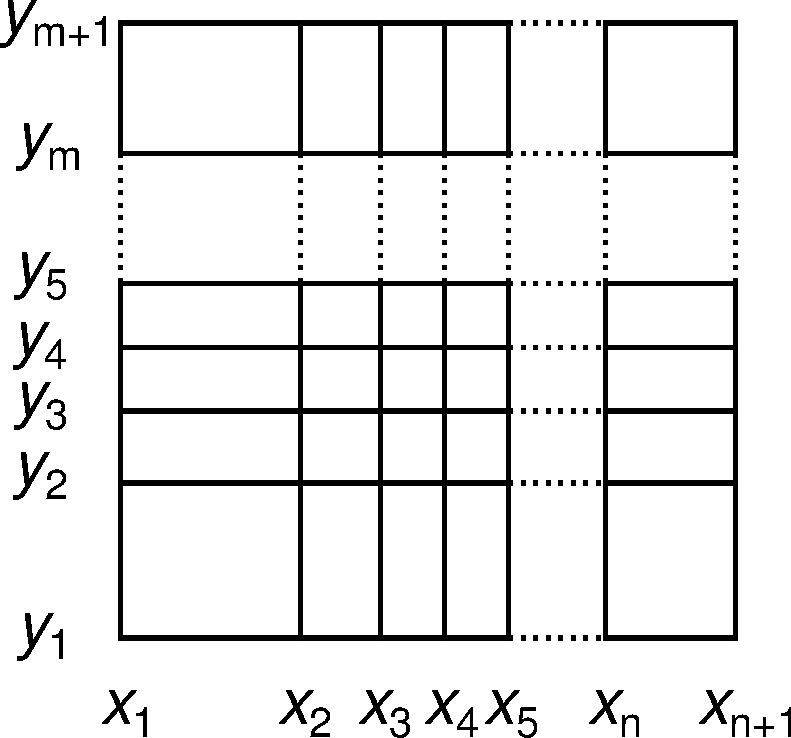
\includegraphics[width=0.4\textwidth]{Octave_PVMOS_Mesh_Topology}
\caption{\label{meshtopo}The mesh topology of meshes created by mkpvmosmesh.}
\end{figure}

The fields in the area definition struct are presented in Table \ref{areadefstruct}. Within the area definition struct there is a struct array of the connection struct, describing the inter electrode connections. The connection struct fields are listed and described in \ref{connstruct}
\begin{table}[H]
\caption{\label{areadefstruct}The fields in the area definition struct}
\begin{longtable}{lrlp{0.4\textwidth}}
Field & Default Value & Unit & Description\\
\hline
name 	& ``default'' 	& - 						& String with the area name. Take care that the names should be unique!\\
Rel	 	&  1 			& [$\Omega$] 				& Array of length \texttt{Nel} with the sheet resistance of each electrode.\\
Rvp	 	&  -1 			& [$\Omega \text{cm}^2$] 	& Array of length \texttt{Nel} with the resistance to the positive node (external voltage source). If the value is negative the elements will have no direct connection to the external source.\\
Rvn	 	&  -1 			& [$\Omega \text{cm}^2$] 	& Array of length \texttt{Nel} with the resistance to the ground node (external voltage source). If the value is negative the elements will have no direct connection to the external source.\\
T		&	300			& [K]						& Scalar value for the temperature in the area\\
SplitX	&	1			& -							& Boolean value (0 is false, 1 is true) indicating whether an element can be split in the $x$-direction during adaptive meshing. If set to 0 the element will not be split.\\
SplitY	&	1			& -							& Boolean value (0 is false, 1 is true) indicating whether an element can be split in the $y$-direction during adaptive meshing. If set to 0 the element will not be split.\\
conn	&	-			& -							& Structure array of length \texttt{Nel}-1 with the properties of the connection between the electrodes
\end{longtable}
% \end{table}

% \begin{table}[!h]
\caption{\label{connstruct}The fields in the connection struct}
\begin{longtable}{lrlp{0.4\textwidth}}
Field & Default Value & Unit & Description\\
\hline
model 	& ``ONED'' 		& - 						& String with the model name. Possible models are:
\begin{tabular}{lp{0.2\textwidth}}
ONED & One diode model\\
TWOD & Two diode model\\
PHOTOT & Photo-transistor model\\
JVD & Tabular JV data
\end{tabular}
\\
Jph	 	&  0 			& [$\text{A}\text{cm}^{-2}$]& Photo-current density for the models  ONED, TWOD, and  PHOTOT\\
Rs	 	&  1e-5			& [$\Omega \text{cm}^2$] 	& Series resistance for the models  ONED, TWOD, and  PHOTOT\\
Rsh	 	&  1e3 			& [$\Omega \text{cm}^2$] 	& Shunt resistance for the models  ONED, TWOD, and  PHOTOT\\
J01		&  1e-12		& [$\text{A}\text{cm}^{-2}$]& Dark saturation current for the first diode, used in models ONED and TWOD\\
J02		&  1e-8			& [$\text{A}\text{cm}^{-2}$]& Dark saturation current for the second diode, used in model TWOD\\
nid1	&  1			& [-]						& Ideality factor of the first diode, used in models ONED and TWOD\\
nid2	&  2			& [-]						& Ideality factor of the second diode, used in model TWOD\\
Eg		&  1.2			& [eV]						& Band gap of the diode, used in models ONED and TWOD\\
Jsbc	&  5e-4			& [$\text{A}\text{cm}^{-2}$]& Dark saturation current density of the main BC diode\\
Jsbe	&  5e-15		& [$\text{A}\text{cm}^{-2}$]& Dark saturation current density of the main BE diode \\
Jse	 	&  0 			& [$\text{A}\text{cm}^{-2}$]& Dark satuartion current of the leakage BE diode\\
Jsc	 	&  0 			& [$\text{A}\text{cm}^{-2}$]& Dark satuartion current of the leakage BC diode\\
Nf	 	&  1 			& [-] 						& Main BE diode ideality factor\\
Nr		&  1			& [-]						& Main BC diode ideality factor\\
Ne		&  1.5			& [-]						& Leakage BE diode ideality factor\\
Nc		&  2			& [-]						& Leakage BC diode ideality factor\\\\
Vaf		&  $\infty$		& [V]						& Forward operation Early voltage\\
Var		&  $\infty$		& [V]						& Reverse operation Early voltage\\
Bf		&  3			& [-]						& Forward operation gain\\
EgBE	&  1.2			& [eV]						& Band gap of the BE diodes\\
PhiBC	&  0.3			& [eV]						& Barrier of the BC junction\\
XTIBE	&  3			& [-]						& Temperature dependency of the BE diodes\\
XTIBC	&  3			& [-]						& Temperature dependency of the BC diodes\\
XTIB	&  3			& [-]						& Temperature dependency of the forward gain\\
\end{longtable}
\end{table}

Several commands are provided to ease the use of the mkpvmosmesh command. To initialize the area definition struct array (\texttt{Area\_Def}), the package provides the function:\\ \\
\texttt{Area\_Def=PVMOS\_AreaProperties(Nel)}\\ \\
It initializes the struct array with one area, using the default values listed in Tables \ref{areadefstruct} and \ref{connstruct}.

I feel it is convenient to work with ``selection masks'' when defining new areas. A selection mask is essentially a matrix, with the same size as the \texttt{Area\_Index} matrix, i.e. one matrix element per mesh element, where a 1 selects the element and a 0 not. There are two functions that allow you to use masks to build up the various areas in the \texttt{Area\_Index} matrix and the \texttt{Area\_Def} area definition struct array. The functions are:\\ \\
\texttt{[Area\_Index, Area\_Def]=PVMOS\_SetMask(Area\_Index,Area\_Def, mask, Mask\_Area)}\\
\begin{itemize}
\item{} \texttt{Area\_Index}, A matrix with index numbers, each number referring to one area
\item{} \texttt{Area\_Def}, The area definition struct array describing the properties of each area
\item{} \texttt{mask}, Mesh element selection mask
\item{} \texttt{Mask\_Area}, Area definition struct to apply to the selected elements (i.e. this area definition will be added to the \texttt{Area\_Def} area definition struct array)
\end{itemize}
and \\ \\
\texttt{[Area\_Index, Area\_Def]=PVMOS\_ModifyMask(Area\_Index,Area\_Def, mask, modlist, name)} \\
\\ \\
\begin{itemize}
\item{} \texttt{Area\_Index}, A matrix with index numbers, each number referring to one area
\item{} \texttt{Area\_Def}, The area definition struct array describing the properties of each area
\item{} \texttt{mask}, Mesh element selection mask
\item{} \texttt{modlist}, Cell array specifying the properties to be changed for the given elements
\item{} \texttt{name}, String with the addition to the area names for the selected elements 
\end{itemize}

The difference between the functions is that  \texttt{PVMOS\_SetMask} sets the area for the selected elements and adds one area to the mesh, whereas the \texttt{PVMOS\_ModifyMask} changes only selected properties for the selected elements, creating as many areas as required. The newly created areas keep the name of the area's they were created from but with the addition of the \texttt{name} string at the end of the area name. 


\section{Examples}
In this section I discuss several examples which can be found in the example directory.
\subsection{Monolithically series connected mini-module and a defect}
In the folder \texttt{Examples/ThinFilm} you can find a PVMOS input file \texttt{thin\_film8x8.mos}. This file creates a thin-film \ASI{} mini-module of \Un{8x8}{cm^2} with 8 cells of \Un{1}{cm} wide. In addition the third cell has a defect. This example demonstrates many basic PVMOS operations such as creating new meshes, joining meshes, selecting elements, locally refine the mesh, create new area's, setting parameters for area's, and assigning elements to an area. 
\subsection{Monolithically series connected mini-module and many defects}
This example consists of the files \texttt{thin\_film40x40.mos} and \texttt{Shunts40x40.m}, both located in \texttt{Examples/ThinFilm}. This example depends on GNU Octave. In this example I use the file \texttt{thin\_film40x40.mos} to create a \Un{40x40}{cm^2} module with 40 cells of \Un{1}{cm} wide. The module that is created is defect-free. In the file \texttt{thin\_film40x40.mos} no simulation is run, the script only creates a defect free mesh which is saved to a binary file. The GNU Octave script \texttt{Shunts40x40.m} creates a random distribution of defects and generates PVMOS scripts where these defects are built in. The PVMOS scripts generated by the GNU Octave script start by loading the defect-free mesh and subsequently locally refine the mesh and add shunts. This script demonstrates the simulation of larger systems (and for that reason is best used on a 64 bit operating system and a 64bit PVMOS executable and several GB of memory) and the saving and loading of meshes. 
\subsection{Metal wrap-through module}
This example is located in \texttt{Examples/Pinup}. The example entails the files several files:
\begin{itemize}
\item{\texttt{mkpvmosmesh.oct}} Dynamic library for GNU Octave to write PVMOS meshes. This needs to be compiled from the PVMOS source tree (``make mkpvmosmesh'') and placed in the example directory.
\item{\texttt{generate\_mesh.m}} Generates the mesh from the images listed below using GNU octave 
\item{\texttt{pinup\_frontmetal.png}} Image used by \texttt{generate\_mesh.m} to define the areas where there is metal at the front
\item{\texttt{pinup\_vias.png}} Image used by \texttt{generate\_mesh.m} to define the areas where the front contact is connected to the contact foil through vias
\item{\texttt{pinup\_backisolation.png}} Image used by \texttt{generate\_mesh.m} to define the areas where the back contact is isolating (around the vias)
\item{\texttt{pinup\_back2contactfoil.png}} Image used by \texttt{generate\_mesh.m} to define the areas where the back contact is connected to the contact foil
\item{\texttt{pinup\_foilisolation.png}} Image used by \texttt{generate\_mesh.m} to define the areas where the contact foil is isolating
\item{\texttt{pinup\_contactfoil\_vn.png}} Image used by \texttt{generate\_mesh.m} to define the areas the contact foil is connected to ground
\item{\texttt{pinup\_contactfoil\_vp.png}} Image used by \texttt{generate\_mesh.m} to define the areas where the contact foil is connected to the positive node.
\item{\texttt{pinup.mos}} The PVMOS input file
\end{itemize}
This example demonstrates how a PVMOS mesh can be generated from images using GNU octave where the images are used as selection masks to select elements and change some parameters for these elements. The example simulateds a metal wrap-through solar cell with three electrose, the front electrode (emitter and front metal), the back electrode (metal contact to the base) and a contact foil at the back which contacts the front metal through vias and the back contact. After running the \texttt{generate\_mesh.m} script in GNU Octave a mesh is written to  \texttt{pinup.bin}. This meash is loaded in the PVMOS script \texttt{pinup.mos}. As the mesh is rather large the mesh is first simplified to reduce the number of elements in the mesh without losing resolution in he area definition. After this step the mesh is a tad coarse for simulating the potentials accurately so the mesh is refined again but this time only there where mesh refinement is needed for an accurate simulation of the potentials. After that the device IV characteristics are simulated.
\subsection{Crystalline silicon module}
The final example is perhaps the most elaborate. In \texttt{Examples/CSiSTD} we do a simulation of a crystalline solar cell with three bus-bars. The simulation extensively uses the definition of new meshes which are glued together to form bigger and more complicated meshes until we have a complete cell with bus-bars and fingers and tabbing wires. It uses all the tricks PVMOS has to generate a complicated geometry from scratch without aid from GNU Octave. The result is a mesh that is comparatively small and therefore allows to do the simulation is a comparatively small memory footprint (less than 0.5 GB) which makes this example even suitable for 32bit machines. There is an optional section in the input file which you can un-comment to simulate the effect of Banksy spray-painting a rat on your solar cell leaving a permanent rat-shaped shadow pattern on the cell. 
\begin{thebibliography}{10}

\bibitem{pvmos:2014}
B.~E. Pieters, ``{PVMOS: A Free and Open Source Simulation Tool for Solar Modules},'' \emph{submitted to: Solar Energy Materials and Solar Cells}, 2015.

\bibitem{Davis:2007:Online}
T.~A. Davis. (retrieved 22 May 2014) {BLAS performance bug and its effect on
  sparse "bench" in MATLAB 7.4}. [Online]. Available:
  \url{http://www.cise.ufl.edu/research/sparse/cholmod/blasbug.html}
\end{thebibliography}
% that's all folks
\end{document}
